%!TEX root = ../ICR.tex
\chapter{Metodología \label{cap:Metodologia}}

En este capítulo se presenta una metodología unificada e integrada para abordar el problema de la detección de noticias falsas en español. La estrategia metodológica se fundamenta en un proceso evolutivo de desarrollo y evaluación que avanza desde técnicas clásicas hasta modelos de lenguaje de última generación, permitiendo una comparación sistemática y objetiva de diferentes paradigmas de inteligencia artificial sobre una base de datos común.

El diseño metodológico adopta un enfoque experimental escalonado que incluye: (1) adquisición y procesamiento unificado de datos, (2) implementación de un pipeline de procesamiento común, (3) desarrollo paralelo de modelos de clasificación utilizando algoritmos metaheurísticos y modelos Transformer, y (4) evaluación comparativa integral bajo un marco de métricas unificado. Este proceso culmina con la implementación de la solución más efectiva en una aplicación web funcional.

\section{Visión General del Proceso Metodológico Integrado}

La metodología se estructura como un pipeline experimental unificado que evalúa sistemáticamente dos paradigmas de inteligencia artificial complementarios. Como se ilustra en la Figura \ref{fig:metodologia_general}, ambos enfoques parten de una base metodológica común pero implementan estrategias de modelado diferenciadas, convergiendo finalmente en una evaluación comparativa que determina la solución óptima.

\textbf{Fundamento del enfoque evolutivo:} Esta investigación adopta una filosofía de desarrollo evolutivo donde se exploran técnicas de complejidad creciente, comenzando con métodos clásicos de PLN optimizados mediante metaheurísticas (estableciendo una línea base sólida) y progresando hacia modelos Transformer de última generación. Esta progresión permite:

\begin{itemize}
    \item \textbf{Validación incremental:} Cada fase valida y mejora los resultados de la anterior
    \item \textbf{Comparación objetiva:} Todos los modelos se evalúan bajo las mismas condiciones experimentales
    \item \textbf{Justificación de complejidad:} Se demuestra empíricamente si la complejidad adicional se traduce en mejoras de rendimiento
    \item \textbf{Transferibilidad metodológica:} Los procesos desarrollados son aplicables a otros tipos de fraude digital
\end{itemize}

Una vez completada la evaluación comparativa, el modelo de mejor rendimiento se implementa en una aplicación web que demuestra la viabilidad práctica de la solución desarrollada.

\begin{figure}[h!]
    \centering
    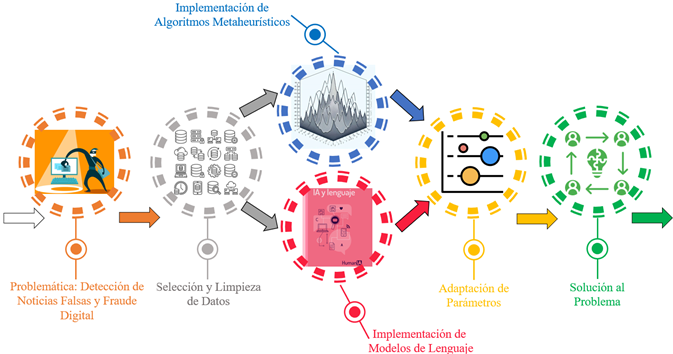
\includegraphics[width=\textwidth]{Imagenes/metodologiaCompleta.png}
    \caption{Metodología propuesta que aborda la problemática combinando Algoritmos Metaheurísticos y Modelos de Lenguaje.}
    \label{fig:metodologia_general}
\end{figure}

\section{Definición y Distinción de Conceptos Fundamentales}
\label{sec:definicion_conceptos}

Antes de proceder con la descripción metodológica, es fundamental establecer con precisión la terminología utilizada en esta investigación, particularmente la distinción entre conceptos relacionados pero diferenciados que a menudo se utilizan de manera intercambiable en la literatura.

\subsection{Distinción entre Noticia Falsa y Bulo}

En el contexto de esta investigación, es esencial distinguir entre dos conceptos fundamentales que, aunque relacionados, poseen características distintivas importantes para el desarrollo de sistemas de detección automática.

% Definir colores adicionales para las tablas de conceptos
\definecolor{LightGreen}{RGB}{144, 238, 144}
\definecolor{LightCoral}{RGB}{240, 128, 128}
\definecolor{LightSkyBlue}{RGB}{135, 206, 250}
\definecolor{LightGoldenrod}{RGB}{250, 250, 210}
\definecolor{LightPink}{RGB}{255, 182, 193}


\subsection{Taxonomía de la Desinformación}

Para proporcionar un marco conceptual completo, esta investigación adopta la taxonomía establecida por la literatura internacional \cite{bondielli2019survey, hu2022deep}, que clasifica el contenido engañoso en tres categorías principales:

\begin{enumerate}
    \item \textbf{\gls{desinformacion}}: Información falsa creada y compartida deliberadamente con intención maliciosa
    \item \textbf{\gls{misinformacion}}: Información incorrecta compartida sin intención maliciosa
    \item \textbf{\gls{malinformacion}}: Información genuina compartida con intención de causar daño
\end{enumerate}

El alcance de esta investigación se centra específicamente en la detección automática de \textbf{desinformación}, abarcando tanto noticias falsas como bulos, reconociendo que ambos tipos requieren estrategias de procesamiento de lenguaje natural diferenciadas pero complementarias.

\subsection{Justificación de la Unificación Terminológica}

En el contexto del desarrollo de sistemas automáticos de detección, la distinción entre noticia falsa y bulo, aunque conceptualmente importante, se aborda mediante un enfoque unificado de \textbf{detección de contenido desinformativo}. Esta decisión metodológica se fundamenta en:

\begin{itemize}
    \item \textbf{Características textuales compartidas}: Ambos tipos utilizan patrones lingüísticos identificables mediante técnicas de PLN
    \item \textbf{Objetivo común}: La finalidad de engañar o desinformar a la audiencia
    \item \textbf{Impacto social similar}: Efectos negativos en la percepción pública y toma de decisiones
    \item \textbf{Necesidad práctica}: Los sistemas de detección automática deben ser capaces de identificar ambos tipos
\end{itemize}

Por tanto, en el resto de este documento, el término \textbf{``noticias falsas''} se utilizará de manera inclusiva para referirse a cualquier tipo de contenido desinformativo, reconociendo la diversidad de formatos y estrategias de propagación que abarca esta categorización.

\subsection{Esquema de Clasificación: Enfoque Binario}
\label{subsec:esquema_clasificacion}

\textbf{Esta investigación adopta un esquema de clasificación binaria}, donde cada noticia se etiqueta en una de dos clases mutuamente excluyentes:

\begin{itemize}
    \item \textbf{Clase 0 (FALSO):} Incluye todo contenido desinformativo, abarcando tanto noticias falsas formales como bulos informales, contenido satírico deliberadamente engañoso, y cualquier tipo de información con intención de desinformar
    \item \textbf{Clase 1 (REAL):} Incluye contenido periodístico legítimo, noticias verificadas de fuentes confiables, y información factualmente correcta
\end{itemize}

\subsubsection{Justificación del Enfoque Binario}

La decisión de utilizar clasificación binaria, en lugar de esquemas multiclase más granulares, se fundamenta en:

\begin{enumerate}
    \item \textbf{Practicidad para usuarios finales:} En aplicaciones reales, los usuarios necesitan una respuesta clara y directa sobre la confiabilidad del contenido
    \item \textbf{Consistencia con la literatura:} La mayoría de trabajos en detección de noticias falsas utilizan esquemas binarios, facilitando la comparación de resultados
    \item \textbf{Robustez del modelo:} Los esquemas binarios tienden a ser más robustos y menos propensos al sobreajuste que las clasificaciones multiclase complejas
    \item \textbf{Disponibilidad de datos:} Los corpus disponibles están mayoritariamente etiquetados de forma binaria
\end{enumerate}

\subsubsection{Consideraciones sobre Esquemas Alternativos}

Aunque este trabajo adopta clasificación binaria, es importante reconocer que existen esquemas alternativos más granulares:

\begin{itemize}
    \item \textbf{Clasificación ternaria:} FALSO, REAL, PARCIALMENTE\_CIERTO
    \item \textbf{Clasificación por niveles de confianza:} Escalas de 5 o 7 puntos de credibilidad
    \item \textbf{Clasificación por tipo de desinformación:} Distinguiendo entre sátira, propaganda, clickbait, etc.
\end{itemize}

Sin embargo, estos enfoques requieren corpus más especializados y presentan desafíos adicionales en términos de consistencia de etiquetado y acuerdo entre anotadores.

\subsection{Fronteras Difusas en la Clasificación de Veracidad}
\label{subsec:fronteras_difusas}

\textbf{Es importante reconocer que la clasificación binaria de contenido informativo presenta inherentemente zonas grises y fronteras difusas}, donde la distinción entre ``verdadero'' y ``falso'' no es absoluta. Esta complejidad conceptual representa uno de los desafíos fundamentales en la detección automatizada de desinformación.

\subsubsection{Casos Límite y Ambigüedades}

En la práctica, existen varios tipos de contenido que desafían la clasificación binaria estricta:

\begin{itemize}
    \item \textbf{Información parcialmente correcta:} Noticias que contienen algunos hechos verificables mezclados con información falsa o tergiversada
    \item \textbf{Contenido satírico ambiguo:} Material humorístico que puede ser malinterpretado como información factual
    \item \textbf{Opiniones presentadas como hechos:} Contenido subjetivo que se presenta con apariencia de objetividad periodística
    \item \textbf{Información desactualizada:} Noticias que fueron ciertas en el pasado pero ya no son válidas
    \item \textbf{Interpretaciones sesgadas:} Presentación de hechos reales con marcos interpretativos tendenciosos
    \item \textbf{Información especulativa:} Predicciones o análisis presentados como hechos consumados
\end{itemize}

\subsubsection{Implicaciones para el Modelado}

Esta ambiguidad inherente se aborda en esta investigación mediante:

\begin{enumerate}
    \item \textbf{Criterios de etiquetado conservadores:} En casos ambiguos, se prioriza la asignación a la clase ``REAL'' para evitar censura inadecuada de contenido legítimo
    \item \textbf{Umbral de confianza:} El modelo genera probabilidades que pueden interpretarse como niveles de certeza, permitiendo identificar casos limítrofes
    \item \textbf{Validación humana en casos dudosos:} Los corpus utilizados fueron validados manualmente para resolver ambigüedades
    \item \textbf{Reconocimiento de limitaciones:} Se asume que un porcentaje mínimo de casos será inherentemente ambiguo y difícil de clasificar con certeza absoluta
\end{enumerate}

\subsubsection{Justificación Pragmática del Enfoque Binario}

A pesar de estas complejidades, el enfoque binario se justifica porque:

\begin{itemize}
    \item \textbf{Utilidad práctica:} Los usuarios finales requieren decisiones claras sobre la credibilidad del contenido
    \item \textbf{Viabilidad técnica:} Los modelos binarios son más robustos y fáciles de entrenar que los esquemas multiclase complejos
    \item \textbf{Consistencia metodológica:} Permite comparación directa con la literatura existente
    \item \textbf{Escalabilidad:} Facilita la anotación y validación de grandes volúmenes de datos
\end{itemize}

Es fundamental entender que \textbf{la frontera difusa no es una limitación del modelo, sino una característica inherente del problema mismo}, que debe ser gestionada mediante diseño metodológico cuidadoso y reconocimiento explícito de las limitaciones del enfoque adoptado.

\section{Construcción del Corpus Unificado}
\label{sec:construccion_corpus}

El primer y más fundamental paso de la metodología fue la construcción de un corpus de alta calidad y de tamaño significativo en español, dada la escasez documentada de recursos centralizados para esta tarea \cite{hu2022deep}.

\begin{table}[htbp]
\centering
\adjustbox{width=\textwidth,center}{%
\footnotesize
\begin{tabular}{|c|l|l|c|c|l|c|}
\hline
\rowcolor{UAMPurple!20}
\textbf{Aspecto} & \textbf{Noticia Falsa} & \textbf{Bulo} \\
\hline
\rowcolor{LightGreen!30}
\textbf{Definición} & 
Información deliberadamente fabricada que se presenta como noticia legítima, pero contiene datos falsos, inexactos o engañosos & 
Información falsa que circula ampliamente, especialmente en redes sociales, con propósito de engañar a la audiencia \\
\hline
\rowcolor{LightSkyBlue!30}
\textbf{Formato} & 
Apariencia de contenido periodístico real, formato de noticia tradicional con titular, cuerpo, fecha, fuente & 
No necesariamente formato periodístico, puede ser texto libre, memes, cadenas de WhatsApp \\
\hline
\rowcolor{LightCoral!30}
\textbf{Intención} & 
Intención maliciosa de desinformar simulando legitimidad periodística & 
Propósito de engañar que apela más a emociones que a hechos verificables \\
\hline
\rowcolor{LightGoldenrod!30}
\textbf{Propagación} & 
Se distribuye a través de sitios web que simulan medios legítimos o plataformas de noticias & 
Circulación viral en redes sociales, aplicaciones de mensajería, cadenas de reenvío \\
\hline
\rowcolor{LightPink!30}
\textbf{Ejemplos} & 
Artículos con titular sensacionalista, byline falso, citas inventadas, estadísticas manipuladas & 
Teorías conspirativas, información médica falsa, rumores políticos, cadenas de ``urgente'' \\
\hline
\rowcolor{HeaderBlue!20}
\textbf{Relevancia para PLN} & 
Estructura textual más predecible, patrones estilísticos identificables en el análisis automatizado & 
Variabilidad estructural mayor, requiere análisis semántico y contextual más sofisticado \\
\hline
\end{tabular}
}
\caption{Comparación detallada entre noticia falsa y bulo en el contexto de detección automática.}
\label{tab:noticia_falsa_vs_bulo}
\end{table}



% Definir colores adicionales para hacer las tablas más coloridas
\definecolor{LightGreen}{RGB}{144, 238, 144}
\definecolor{LightCoral}{RGB}{240, 128, 128}
\definecolor{LightSkyBlue}{RGB}{135, 206, 250}
\definecolor{LightGoldenrod}{RGB}{250, 250, 210}
\definecolor{LightPink}{RGB}{255, 182, 193}

\subsection{Fuentes de Datos Académicas}

Se llevó a cabo un proceso exhaustivo de investigación y unificación de cuatro corpus académicos reconocidos, los cuales constituyen pilares en la investigación de noticias falsas en español. \textbf{Es importante señalar que, aunque todos los corpus convergen hacia el objetivo común de detección de desinformación, cada uno fue desarrollado con enfoques metodológicos y propósitos específicos diferentes}, lo que enriquece la diversidad y robustez del conjunto de datos unificado. La Tabla \ref{tab:corpus_academicos} presenta un resumen detallado de estos recursos y sus características distintivas.

\begin{table}[htbp]
\centering
\adjustbox{width=\textwidth,center}{%
\footnotesize
\begin{tabular}{|c|l|l|c|c|l|c|}
\hline
\rowcolor{UAMPurple!20}
\textbf{ID} & \textbf{Nombre del Corpus} & \textbf{Autores Principales} & \textbf{Año} & \textbf{Noticias} & \textbf{Características} & \textbf{Ref.} \\
\hline
\rowcolor{LightGreen!30}
1 & \begin{tabular}[t]{@{}l@{}}Spanish Fake News Corpus\\(IberLEF)\end{tabular} & \begin{tabular}[t]{@{}l@{}}Posadas-Durán, J.P.\\Gómez-Adorno, H.\end{tabular} & 2019-2021 & 971 & \begin{tabular}[t]{@{}l@{}}Análisis estilométrico\\Múltiples versiones\end{tabular} & \cite{posadas2019detection} \\
\hline
\rowcolor{LightSkyBlue!30}
2 & \begin{tabular}[t]{@{}l@{}}Conjunto de datos Zules Acosta\\(UPM)\end{tabular} & Acosta, F.A.Z. & 2019 & 598 & \begin{tabular}[t]{@{}l@{}}Trabajo fin de maestría\\Extracción web verificada\end{tabular} & \cite{acosta2019construccion} \\
\hline
\rowcolor{LightCoral!30}
3 & \begin{tabular}[t]{@{}l@{}}Conjunto de datos Tretiakov\\(Kaggle)\end{tabular} & \begin{tabular}[t]{@{}l@{}}Tretiakov, A.\\Martín García, A.\end{tabular} & 2022 & 1,958 & \begin{tabular}[t]{@{}l@{}}Aprendizaje automático\\Disponible públicamente\end{tabular} & \cite{tretiakov2022detection} \\
\hline
\rowcolor{LightGoldenrod!30}
4 & \begin{tabular}[t]{@{}l@{}}Spanish Political Fake News\\Conjunto de datos\end{tabular} & \begin{tabular}[t]{@{}l@{}}Blanco-Fernández, Y.\\Otero-Vizoso, J.\end{tabular} & 2024 & 57,231 & \begin{tabular}[t]{@{}l@{}}Temática política\\Modelos BERT/RoBERTa\end{tabular} & \cite{blanco2024enhancing} \\
\hline
\rowcolor{HeaderBlue!20}
\multicolumn{5}{|c|}{\textbf{TOTAL CORPUS ACADÉMICOS}} & \textbf{60,758} & \textbf{Cuatro fuentes} \\
\hline
\end{tabular}
}
\caption{Corpus académicos utilizados para la construcción del conjunto de datos unificado.}
\label{tab:corpus_academicos}
\end{table}

\subsubsection{Spanish Fake News Corpus (IberLEF)}

Este corpus, asociado a las competencias de IberLEF y desarrollado por Posadas-Durán, Gómez-Adorno, et al., ha tenido varias versiones. La versión original y más citada del corpus contiene un total de 971 noticias \cite{posadas2019detection}. \textbf{Su propósito específico fue el desarrollo de técnicas de análisis estilométrico para identificar patrones lingüísticos distintivos en texto desinformativo}. Este corpus se caracteriza por su enfoque metodológico riguroso en análisis estilométrico y ha sido utilizado en múltiples evaluaciones comparativas dentro del marco de las competencias IberLEF \cite{gomez2021overview, aragon2020overview}. \textbf{Las fuentes de este corpus provienen principalmente de sitios web verificados como desinformativos por organismos de verificación de datos españoles y latinoamericanos}. Las versiones posteriores del corpus han sido mantenidas y actualizadas en repositorios públicos \cite{ramirez2021spanish}.

\subsubsection{Conjunto de datos de Zules Acosta (Universidad Politécnica de Madrid)}

Desarrollado como parte de un Trabajo Fin de Maestría Universitaria en Ciberseguridad en la Universidad Politécnica de Madrid, este corpus contiene 598 noticias verificadas \cite{acosta2019construccion}. \textbf{Su propósito original fue establecer una metodología de construcción de corpus para noticias falsas en español, con énfasis en la verificación manual exhaustiva}. El conjunto de datos fue construido mediante técnicas de extracción web y se encuentra disponible públicamente en la plataforma Kaggle \cite{acosta2019dataset, zules2019spanish}. \textbf{Las fuentes incluyen tanto medios legítimos (para noticias reales) como sitios identificados como propagadores de desinformación, con verificación cruzada mediante múltiples verificadores de hechos}. Su contribución principal radica en la aplicación de metodologías rigurosas de verificación para la construcción de conjuntos de datos de noticias falsas.

\subsubsection{Dataset de Tretiakov et al.}

Este corpus, desarrollado por Tretiakov, Martín García y Camacho, contiene 1,958 noticias falsas en español \cite{tretiakov2022detection}. \textbf{Su propósito específico fue la evaluación de técnicas de aprendizaje automático tradicionales para clasificación binaria de contenido desinformativo}. El conjunto de datos fue creado en el contexto de técnicas de aprendizaje automático para la detección de información falsa y se encuentra disponible públicamente en Kaggle \cite{tretiakov2022noticias}. \textbf{Las fuentes de este corpus se concentran en redes sociales y plataformas digitales donde se propaga desinformación, incluyendo Twitter, Facebook y sitios web no verificados}. Su enfoque se centra en la aplicación de técnicas de aprendizaje automático para la clasificación automatizada de contenido desinformativo.

\subsubsection{Spanish Political Fake News Dataset}

El corpus más extenso utilizado, desarrollado por Blanco-Fernández et al., contiene 57,231 noticias de temática política \cite{blanco2024enhancing}. \textbf{Su propósito específico fue evaluar modelos transformer (BERT/RoBERTa) en el dominio político, donde la desinformación tiene particular relevancia social}. Este conjunto de datos fue específicamente diseñado para evaluar modelos BERT y RoBERTa en la detección de desinformación política en español y se encuentra disponible en Kaggle \cite{blanco2024spanish}. \textbf{Las fuentes incluyen tanto medios de comunicación tradicionales como plataformas digitales especializadas en contenido político, con particular énfasis en el contexto español e iberoamericano}. Su gran tamaño y enfoque en contenido político lo convierte en un recurso valioso para el entrenamiento de modelos de gran escala.

\subsection{Análisis Comparativo Detallado de los Corpus Utilizados}

Para garantizar una comprensión completa de las características y diferencias entre los corpus utilizados, se presenta un análisis comparativo exhaustivo que permite entender las fortalezas y limitaciones de cada fuente de datos, así como las decisiones metodológicas tomadas en el proceso de unificación.

\begin{table}[htbp]
\centering
\adjustbox{width=\textwidth,center}{%
\tiny
\begin{tabular}{|l|c|c|c|c|c|}
\hline
\rowcolor{UAMPurple!20}
\textbf{Aspecto Comparativo} & \textbf{Posadas-Durán} & \textbf{Acosta (UPM)} & \textbf{Tretiakov} & \textbf{Blanco-Fernández} & \textbf{El Deforma} \\
\hline
\rowcolor{LightBlue!30}
\textbf{Tamaño del corpus} & 971 noticias & 598 noticias & 1,958 noticias & 57,231 noticias & 9,000 noticias \\
\hline
\rowcolor{LightGreen!30}
\textbf{Año de creación} & 2019-2021 & 2019 & 2022 & 2024 & 2024 (extracción) \\
\hline
\rowcolor{LightYellow!30}
\textbf{Enfoque metodológico} & 
\begin{tabular}[t]{@{}l@{}}Análisis estilométrico\\Competencias IberLEF\end{tabular} & 
\begin{tabular}[t]{@{}l@{}}Metodología de\\construcción de corpus\end{tabular} & 
\begin{tabular}[t]{@{}l@{}}Aprendizaje automático\\tradicional\end{tabular} & 
\begin{tabular}[t]{@{}l@{}}Modelos Transformer\\BERT/RoBERTa\end{tabular} & 
\begin{tabular}[t]{@{}l@{}}Contenido satírico\\Web scraping\end{tabular} \\
\hline
\rowcolor{LightCoral!30}
\textbf{Dominio temático} & General & General & General & Político específico & Satírico/General \\
\hline
\rowcolor{LightPink!30}
\textbf{Distribución de clases} & Balanceado & Balanceado & Solo falsas & Balanceado & Solo falsas \\
\hline
\rowcolor{LightOrange!30}
\textbf{Fuentes de noticias reales} & 
\begin{tabular}[t]{@{}l@{}}Medios españoles\\verificados\end{tabular} & 
\begin{tabular}[t]{@{}l@{}}Múltiples medios\\internacionales\end{tabular} & 
N/A & 
\begin{tabular}[t]{@{}l@{}}Medios políticos\\españoles\end{tabular} & 
N/A \\
\hline
\rowcolor{LightGray!30}
\textbf{Fuentes de noticias falsas} & 
\begin{tabular}[t]{@{}l@{}}Sitios verificados como\\desinformativos\end{tabular} & 
\begin{tabular}[t]{@{}l@{}}Fact-checkers y\\verificadores\end{tabular} & 
\begin{tabular}[t]{@{}l@{}}Redes sociales y\\sitios no verificados\end{tabular} & 
\begin{tabular}[t]{@{}l@{}}Desinformación\\política verificada\end{tabular} & 
\begin{tabular}[t]{@{}l@{}}Portal satírico\\El Deforma\end{tabular} \\
\hline
\rowcolor{LightBlue!30}
\textbf{Variabilidad regional} & España/Latinoamérica & Internacional & Múltiple & España & México \\
\hline
\rowcolor{LightGreen!30}
\textbf{Periodo temporal} & 2018-2021 & 2018-2019 & 2020-2022 & 2020-2024 & 2020-2024 \\
\hline
\rowcolor{LightYellow!30}
\textbf{Calidad de anotación} & 
\begin{tabular}[t]{@{}l@{}}Alta - múltiples\\anotadores\end{tabular} & 
\begin{tabular}[t]{@{}l@{}}Alta - verificación\\manual exhaustiva\end{tabular} & 
\begin{tabular}[t]{@{}l@{}}Media - basada\\en fuentes\end{tabular} & 
\begin{tabular}[t]{@{}l@{}}Alta - verificación\\política especializada\end{tabular} & 
\begin{tabular}[t]{@{}l@{}}Automática - contenido\\inherentemente falso\end{tabular} \\
\hline
\rowcolor{LightCoral!30}
\textbf{Metadatos incluidos} & 
\begin{tabular}[t]{@{}l@{}}Características\\estilométricas\end{tabular} & 
\begin{tabular}[t]{@{}l@{}}Fuente, fecha,\\categoría\end{tabular} & 
\begin{tabular}[t]{@{}l@{}}Fecha, fuente,\\contexto\end{tabular} & 
\begin{tabular}[t]{@{}l@{}}Orientación política,\\fecha, fuente\end{tabular} & 
\begin{tabular}[t]{@{}l@{}}URL, fecha de\\extracción\end{tabular} \\
\hline
\rowcolor{LightPink!30}
\textbf{Disponibilidad pública} & 
\begin{tabular}[t]{@{}l@{}}GitHub\\(IberLEF)\end{tabular} & 
\begin{tabular}[t]{@{}l@{}}Kaggle\\UPM\end{tabular} & 
\begin{tabular}[t]{@{}l@{}}Kaggle\\Público\end{tabular} & 
\begin{tabular}[t]{@{}l@{}}Kaggle\\Applied Sciences\end{tabular} & 
\begin{tabular}[t]{@{}l@{}}Generado para\\esta tesis\end{tabular} \\
\hline
\rowcolor{LightOrange!30}
\textbf{Fortaleza principal} & 
\begin{tabular}[t]{@{}l@{}}Análisis lingüístico\\profundo\end{tabular} & 
\begin{tabular}[t]{@{}l@{}}Metodología\\rigurosa\end{tabular} & 
\begin{tabular}[t]{@{}l@{}}Foco en ML\\tradicional\end{tabular} & 
\begin{tabular}[t]{@{}l@{}}Gran escala y\\especialización política\end{tabular} & 
\begin{tabular}[t]{@{}l@{}}Contemporaneidad\\y diversidad\end{tabular} \\
\hline
\rowcolor{LightGray!30}
\textbf{Limitación principal} & 
\begin{tabular}[t]{@{}l@{}}Tamaño\\limitado\end{tabular} & 
\begin{tabular}[t]{@{}l@{}}Tamaño muy\\pequeño\end{tabular} & 
\begin{tabular}[t]{@{}l@{}}Solo noticias\\falsas\end{tabular} & 
\begin{tabular}[t]{@{}l@{}}Dominio muy\\específico\end{tabular} & 
\begin{tabular}[t]{@{}l@{}}Solo contenido\\satírico\end{tabular} \\
\hline
\rowcolor{LightBlue!30}
\textbf{Contribución al corpus final} & 1.6\% & 1.0\% & 3.2\% & 92.8\% & 14.6\% \\
\hline
\end{tabular}
}
\caption{Comparación exhaustiva de características de los corpus utilizados en la construcción del conjunto de datos unificado.}
\label{tab:comparacion_exhaustiva_corpus}
\end{table}

\subsubsection{Características de Variabilidad Regional del Español}

Una consideración metodológica fundamental en esta investigación es el reconocimiento y aprovechamiento de la diversidad regional del español presente en los corpus utilizados. \textbf{El corpus unificado representa un enfoque de español neutro multiregional}, lo que constituye una fortaleza metodológica significativa:

\textbf{Distribución geográfica y justificación:}
\begin{itemize}
    \item \textbf{Español peninsular (España):} Representado principalmente en los corpus de Posadas-Durán \cite{posadas2019detection} y Blanco-Fernández \cite{blanco2024enhancing}, que utilizan fuentes de medios españoles verificados
    
    \item \textbf{Español mexicano:} Incorporado a través del contenido de ``El Deforma'' y fuentes mexicanas presentes en el corpus de Acosta \cite{acosta2019construccion}
    
    \item \textbf{Español latinoamericano diverso:} El corpus de Acosta incluye fuentes internacionales que abarcan múltiples países de habla hispana
    
    \item \textbf{Español digital contemporáneo:} Los corpus más recientes (2020-2024) capturan la evolución del español en medios digitales
\end{itemize}

\textbf{Ventajas metodológicas del enfoque multiregional:}
\begin{itemize}
    \item \textbf{Robustez del modelo:} Capacidad de detectar desinformación independientemente de la variante regional
    \item \textbf{Generalización lingüística:} Menor sesgo hacia construcciones específicas de una región
    \item \textbf{Aplicabilidad universal:} El modelo resultante es funcional para toda la comunidad hispanohablante
    \item \textbf{Representatividad real:} Refleja el consumo actual de noticias en español, que frecuentemente cruza fronteras nacionales
\end{itemize}

Esta diversidad regional no constituye una limitación, sino una fortaleza que permite desarrollar modelos más robustos y ampliamente aplicables.

\textbf{1. Diversidad Metodológica:}
\begin{itemize}
    \item \textbf{Corpus de Posadas-Durán:} Aporta rigor en análisis estilométrico y experiencia en competencias académicas
    \item \textbf{Corpus de Acosta:} Contribuye con metodología de construcción verificada manualmente
    \item \textbf{Corpus de Tretiakov:} Añade perspectiva de ML tradicional y fuentes de redes sociales
    \item \textbf{Corpus de Blanco-Fernández:} Proporciona escala masiva y especialización en dominio político
    \item \textbf{Contenido de El Deforma:} Introduce diversidad estilística y contemporaneidad
\end{itemize}

\textbf{2. Cobertura Temporal y Geográfica:}
\begin{itemize}
    \item \textbf{Span temporal:} 2018-2024 (6 años de evolución en patrones de desinformación)
    \item \textbf{Cobertura geográfica:} España, México, Latinoamérica (diversidad regional del español)
    \item \textbf{Evolución temática:} Desde temas generales hasta especialización política y satírica
\end{itemize}

\textbf{3. Complementariedad en Tipos de Desinformación:}
\begin{itemize}
    \item \textbf{Desinformación tradicional:} Corpus académicos con verificación formal
    \item \textbf{Desinformación política:} Especialización del corpus de Blanco-Fernández
    \item \textbf{Contenido satírico:} Ampliación con El Deforma para diversidad estilística
    \item \textbf{Múltiples fuentes:} Desde medios tradicionales hasta redes sociales
\end{itemize}

\textbf{4. Validación de Robustez:}
La diversidad en metodologías de construcción permite validar la robustez de los modelos desarrollados:
\begin{itemize}
    \item Modelos entrenados deben generalizar entre diferentes tipos de anotación
    \item Capacidad de detectar patrones consistentes a pesar de diferencias metodológicas
    \item Evaluación de transferencia entre dominios (general → político → satírico)
\end{itemize}

\subsubsection{Justificación de la Estrategia de Unificación}

La decisión de unificar corpus heterogéneos se basa en varios principios metodológicos sólidos:

\textbf{1. Principio de Máxima Diversidad:}
\begin{itemize}
    \item Mayor variabilidad en patrones lingüísticos
    \item Reducción de sesgos específicos de corpus individuales
    \item Mejora en generalización de modelos entrenados
\end{itemize}

\textbf{2. Principio de Escala Efectiva:}
\begin{itemize}
    \item Aprovechamiento del corpus grande (Blanco-Fernández) como base
    \item Enriquecimiento con corpus especializados más pequeños
    \item Balanceo mediante extracción web controlada
\end{itemize}

\textbf{3. Principio de Validación Cruzada:}
\begin{itemize}
    \item Cada corpus actúa como validación independiente de los otros
    \item Patrones consistentes entre corpus indican robustez
    \item Diferencias señalan áreas que requieren atención especial
\end{itemize}

\subsection{Proceso de Unificación y Estandarización}

La integración de corpus heterogéneos requirió un proceso sistemático de estandarización que incluyó:

\begin{enumerate}
    \item \textbf{Normalización de formato:} Unificación de esquemas de etiquetado en un sistema binario consistente (FALSO=0, REAL=1) y estandarización de estructuras de datos CSV con separador de punto y coma
    \item \textbf{Eliminación de duplicados:} Implementación de algoritmos de detección de contenido similar basados en hash de texto y comparación de títulos
    \item \textbf{Validación de calidad:} Verificación manual de una muestra estadísticamente significativa para confirmar la calidad del etiquetado y consistencia temática
    \item \textbf{Balanceo de clases:} Análisis detallado de la distribución de clases para identificar necesidades de ampliación y garantizar equilibrio. El balanceo se refiere a mantener una proporción similar entre noticias ``FALSAS'' y ``REALES'' (idealmente cercana al 50\%-50\%) para evitar sesgos algorítmicos y garantizar que los modelos aprendan a detectar ambas clases con igual efectividad
    \item \textbf{Limpieza de datos:} Eliminación de registros con valores nulos o inconsistentes mediante \texttt{dropna()} y validación de tipos de datos
\end{enumerate}

\subsection{Ampliación del Corpus Mediante Extracción Web}

Para mejorar el balance del conjunto de datos y aumentar la diversidad de las noticias etiquetadas como ``FALSAS'', se aplicaron técnicas de extracción web automatizada. Se desarrolló un script especializado en Python utilizando las librerías BeautifulSoup y Requests para extraer de forma sistemática los titulares y cuerpos de noticia del portal de contenido satírico ``El Deforma''.

\subsubsection{Proceso de Extracción Web Automatizada}

El proceso de extracción automatizada se ejecutó en múltiples fases para alcanzar el objetivo de 9,000 noticias adicionales. La Tabla \ref{tab:web_scraping_proceso} detalla las diferentes etapas implementadas.

\begin{table}[htbp]
\centering
\adjustbox{width=\textwidth,center}{%
\small
\begin{tabular}{|c|l|l|c|c|l|}
\hline
\rowcolor{UAMPurple!20}
\textbf{Fase} & \textbf{Estrategia} & \textbf{Técnica Utilizada} & \textbf{Objetivo} & \textbf{Resultado} & \textbf{Observaciones} \\
\hline
\rowcolor{LightGreen!30}
1 & Scraping Inicial & \begin{tabular}[t]{@{}l@{}}Navegación por enlaces\\Extracción de contenido\end{tabular} & 1,000 & 1,000 & \begin{tabular}[t]{@{}l@{}}Proceso exitoso\\Base establecida\end{tabular} \\
\hline
\rowcolor{LightSkyBlue!30}
2 & \begin{tabular}[t]{@{}l@{}}Búsqueda Expandida\\Masiva\end{tabular} & \begin{tabular}[t]{@{}l@{}}URLs desde existentes\\Crawling híbrido\end{tabular} & 9,000 & 2,495 & \begin{tabular}[t]{@{}l@{}}Expansión limitada\\Nuevas estrategias\end{tabular} \\
\hline
\rowcolor{LightCoral!30}
3 & \begin{tabular}[t]{@{}l@{}}Crawler Híbrido\\Persistente\end{tabular} & \begin{tabular}[t]{@{}l@{}}URLs semilla\\Trafilatura\end{tabular} & 9,000 & 2,495 & \begin{tabular}[t]{@{}l@{}}Estabilización\\Mismo resultado\end{tabular} \\
\hline
\rowcolor{LightGoldenrod!30}
4 & \begin{tabular}[t]{@{}l@{}}Paginación\\Sistemática\end{tabular} & \begin{tabular}[t]{@{}l@{}}Escaneo por páginas\\Indexación completa\end{tabular} & 9,000 & 9,000 & \begin{tabular}[t]{@{}l@{}}Éxito completo\\Objetivo alcanzado\end{tabular} \\
\hline
\rowcolor{HeaderBlue!20}
\multicolumn{4}{|c|}{\textbf{TOTAL EXTRAÍDO}} & \textbf{9,000} & \textbf{Extracción web completada} \\
\hline
\end{tabular}
}
\caption{Fases del proceso de extracción web implementado para ``El Deforma''.}
\label{tab:web_scraping_proceso}
\end{table}

\subsubsection{Implementación Técnica de la Extracción Web}

El proceso de extracción automatizada incluyó:

\begin{enumerate}
    \item \textbf{Identificación de patrones:} Análisis de la estructura HTML del sitio web objetivo para identificar selectores CSS consistentes (\texttt{h1.tdb-title-text}, \texttt{div.tdb-block-inner})
    \item \textbf{Extracción automatizada:} Implementación de rutinas de extracción con manejo de errores y delays aleatorios (1.5-4.5 segundos) para evitar sobrecarga del servidor
    \item \textbf{Validación de contenido:} Verificación automática de la calidad del contenido extraído mediante filtros de longitud mínima (500 caracteres)
    \item \textbf{Limpieza de texto:} Eliminación de disclaimers específicos del sitio, caracteres especiales y normalización de espacios mediante expresiones regulares
    \item \textbf{Etiquetado automático:} Asignación de etiqueta ``FALSO'' (0) a todo el contenido extraído del portal satírico
    \item \textbf{Persistencia progresiva:} Guardado en lotes de 50 registros con formato CSV y separador de punto y coma para evitar pérdida de datos
    \item \textbf{Gestión de estado:} Implementación de archivos de progreso para permitir la reanudación del proceso en caso de interrupción
\end{enumerate}

La Tabla \ref{tab:corpus_referencias_completas} presenta las referencias bibliográficas completas de todos los corpus utilizados, organizadas por tipo de fuente.

\begin{table}[htbp]
\centering
\adjustbox{width=\textwidth,center}{%
\footnotesize
\begin{tabular}{|l|l|l|c|}
\hline
\rowcolor{UAMPurple!20}
\textbf{\textcolor{white}{Corpus}} & \textbf{\textcolor{white}{Tipo de Referencia}} & \textbf{\textcolor{white}{Fuente Principal}} & \textbf{\textcolor{white}{Referencia}} \\
\hline
\rowcolor{LightGreen}
\textbf{Spanish Fake News Corpus (IberLEF)} & Artículo original & Journal of Intelligent and Fuzzy Systems & \cite{posadas2019detection} \\
\hline
\rowcolor{ProfessionalGray}
Spanish Fake News Corpus (IberLEF) & Workshop IberLEF 2021 & Procesamiento del Lenguaje Natural & \cite{gomez2021overview} \\
\hline
\rowcolor{ProfessionalGray}
Spanish Fake News Corpus (IberLEF) & Workshop IberLEF 2020 & IberLEF Workshop Proceedings & \cite{aragon2020overview} \\
\hline
\rowcolor{ProfessionalGray}
Spanish Fake News Corpus (IberLEF) & Repositorio GitHub & GitHub Repository & \cite{ramirez2021spanish} \\
\hline
\rowcolor{LightBlue}
\textbf{Conjunto de datos Zules Acosta (UPM)} & Tesis de Maestría & Universidad Politécnica de Madrid & \cite{acosta2019construccion} \\
\hline
\rowcolor{ProfessionalGray}
Dataset Zules Acosta (UPM) & Dataset Kaggle & Kaggle Platform & \cite{zules2019spanish} \\
\hline
\rowcolor{LightCoral}
\textbf{Dataset Tretiakov (Kaggle)} & Capítulo de libro & Springer Book Chapter & \cite{tretiakov2022detection} \\
\hline
\rowcolor{ProfessionalGray}
Dataset Tretiakov (Kaggle) & Dataset Kaggle & Kaggle Platform & \cite{tretiakov2022noticias} \\
\hline
\rowcolor{LightGold}
\textbf{Spanish Political Fake News Dataset} & Artículo científico & Applied Sciences Journal & \cite{blanco2024enhancing} \\
\hline
\rowcolor{ProfessionalGray}
Spanish Political Fake News Dataset & Dataset Kaggle & Kaggle Platform & \cite{blanco2024spanish} \\
\hline
\end{tabular}
}
\caption{Referencias bibliográficas completas de los corpus académicos utilizados.}
\label{tab:corpus_referencias_completas}
\end{table}

La estrategia final exitosa utilizó paginación sistemática, escaneando secuencialmente desde \texttt{https://eldeforma.com/page/1/} hasta alcanzar las 9,000 noticias objetivo, garantizando cobertura completa del contenido disponible.

Esta estrategia de ampliación se justifica por varios factores:
\begin{itemize}
    \item \textbf{Diversidad estilística:} Incorporación de diferentes estilos de contenido falso o satírico
    \item \textbf{Volumen de datos:} Incremento significativo del conjunto de entrenamiento
    \item \textbf{Actualidad temporal:} Inclusión de contenido contemporáneo que refleja tendencias actuales
    \item \textbf{Variabilidad temática:} Ampliación del espectro de temas cubiertos en el corpus
\end{itemize}

\subsection{Corpus Final y Estrategia de División}

El proceso completo de unificación, limpieza de duplicados y ampliación mediante extracción web resultó en un \textbf{corpus final con 61,674 noticias únicas}, constituyendo uno de los recursos más extensos disponibles para la detección de noticias falsas en español.

\subsubsection{Análisis de Composición Final}

La Tabla \ref{tab:corpus_final} presenta la composición detallada del corpus unificado final.

\begin{table}[htbp]
\centering
\adjustbox{width=0.9\textwidth,center}{%
\begin{tabular}{|l|c|c|c|c|}
\hline
\rowcolor{UAMPurple!20}
\textbf{Fuente de Datos} & \textbf{Noticias} & \textbf{Porcentaje} & \textbf{Tipo} & \textbf{Estado} \\
\hline
\rowcolor{LightGreen!30}
Corpus Académicos Unificados & 52,689 & 85.4\% & Mixto & Procesado \\
\hline
\rowcolor{LightPink!30}
Extracción Web ``El Deforma'' & 9,000 & 14.6\% & Falso & Extraído \\
\hline
\rowcolor{LightCoral!30}
Duplicados Eliminados & -15 & -0.02\% & -- & Removido \\
\hline
\rowcolor{HeaderBlue!20}
\textbf{CORPUS FINAL} & \textbf{61,674} & \textbf{100\%} & \textbf{Balanceado} & \textbf{Listo} \\
\hline
\end{tabular}
}
\caption{Composición final del corpus unificado después del procesamiento completo.}
\label{tab:corpus_final}
\end{table}

El análisis de balance del corpus final mostró una distribución equilibrada:
\begin{itemize}
    \item \textbf{Noticias FALSAS (0):} 30,734 registros (49.8\%)
    \item \textbf{Noticias REALES (1):} 30,940 registros (50.2\%)
\end{itemize}

\subsubsection{Concepto y Importancia del Balanceo de Clases}

El \textbf{balanceo de clases} es un concepto fundamental en el aprendizaje automático que se refiere a la distribución equitativa de ejemplos entre las diferentes categorías o clases del conjunto de datos. En el contexto de la detección de noticias falsas, esto significa mantener una proporción similar entre noticias etiquetadas como ``FALSAS'' y ``REALES''.

\textbf{¿Por qué es crucial el balanceo?}

\begin{enumerate}
    \item \textbf{Prevención de sesgo algorítmico:} Un conjunto de datos desbalanceado puede llevar a que el modelo aprenda a predecir sistemáticamente la clase mayoritaria, ignorando la minoritaria
    \item \textbf{Métricas de evaluación confiables:} Las métricas como exactitud pueden ser engañosas en datasets desbalanceados (ejemplo: 95\% de exactitud puede significar que el modelo siempre predice la clase mayoritaria)
    \item \textbf{Generalización robusta:} Los modelos entrenados con datos balanceados tienden a generalizar mejor en escenarios reales donde la distribución puede ser diferente
    \item \textbf{Detección efectiva de ambas clases:} Es igualmente importante detectar noticias falsas como preservar noticias verdaderas
\end{enumerate}

\textbf{Estrategias implementadas para lograr el balanceo:}

\begin{itemize}
    \item \textbf{Análisis cuantitativo inicial:} Evaluación de la distribución de clases en cada corpus individual
    \item \textbf{Identificación de déficits:} Detección de desbalances significativos que requerían corrección
    \item \textbf{Extracción web dirigida:} Adición estratégica de 9,000 noticias falsas mediante web scraping para compensar el déficit
    \item \textbf{Validación final:} Confirmación de que la distribución resultante es prácticamente equilibrada (49.8\% vs 50.2\%)
\end{itemize}

\begin{figure}[htbp]
    \centering
    % TODO: Agregar imagen que muestre:
    % - Gráfico de barras comparando distribución antes y después del balanceo
    % - Visualización de la proporción 49.8% vs 50.2%
    % - Comparación con ejemplos de datasets desbalanceados (ej: 80%-20%)
    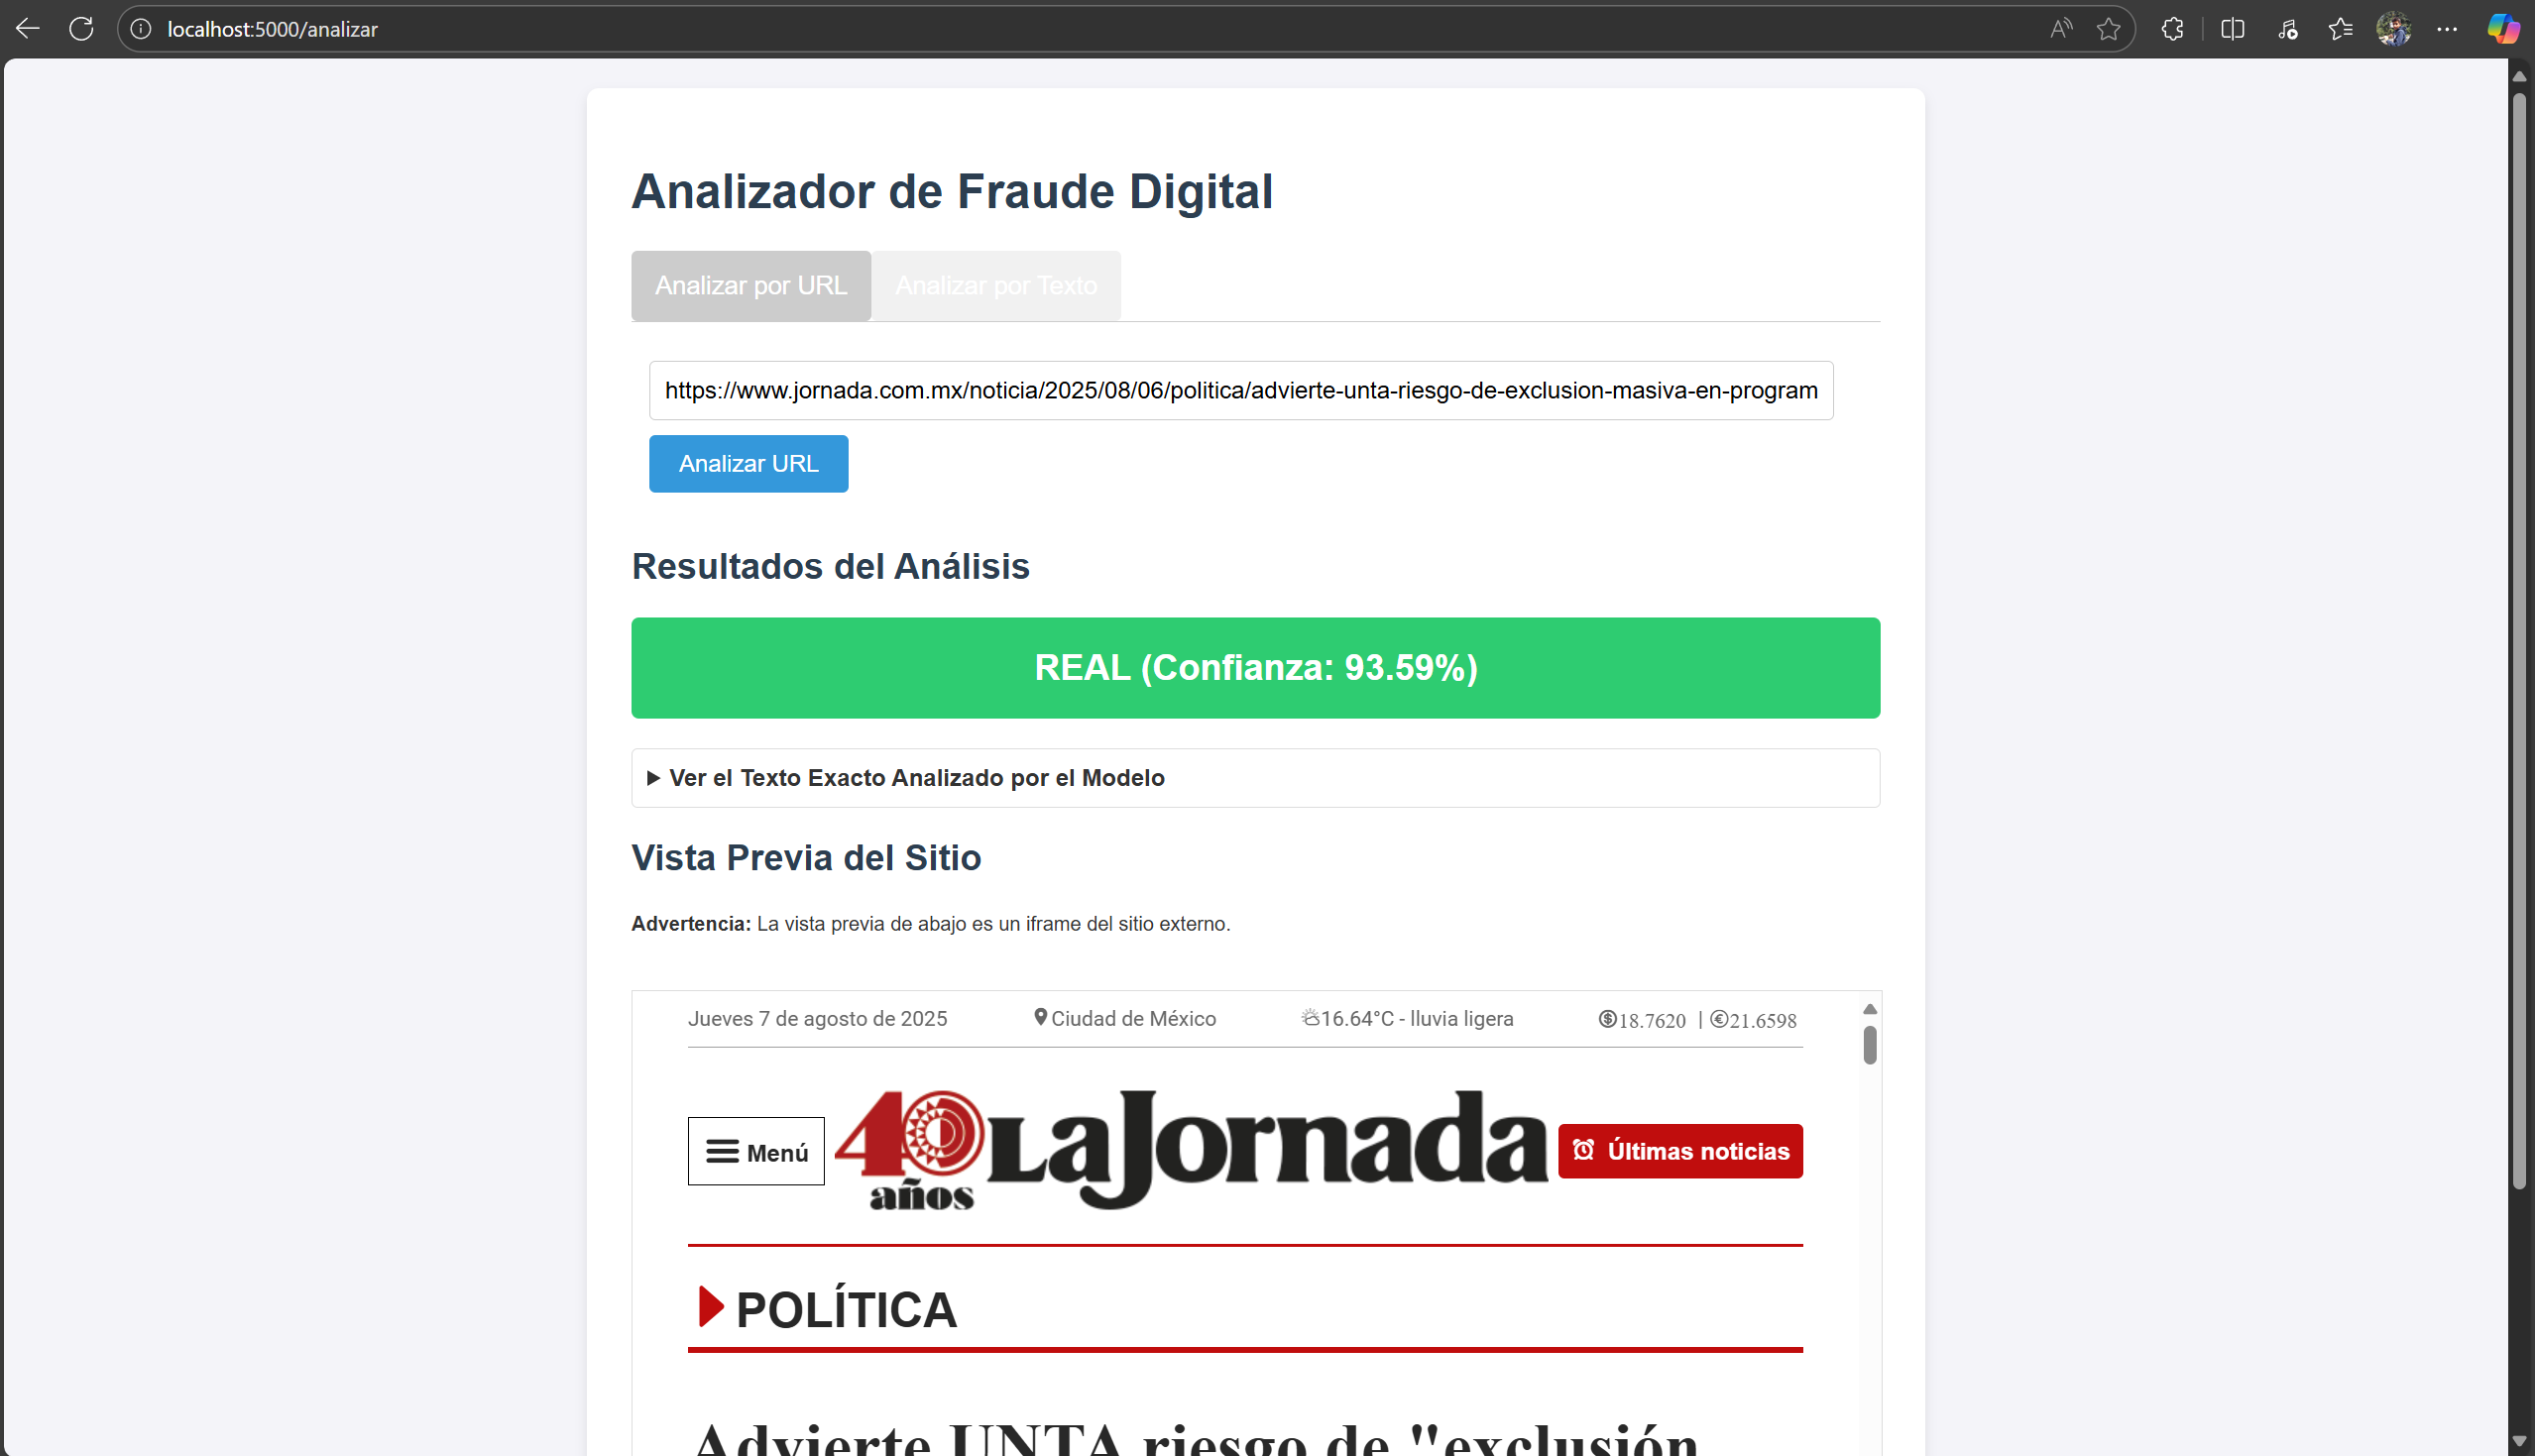
\includegraphics[width=0.8\textwidth]{Imagenes/balanceo_corpus_explicacion.png}
    \caption{Representación gráfica del proceso de balanceo del corpus: comparación entre distribución inicial desbalanceada y distribución final equilibrada. La imagen muestra cómo la extracción web de 9,000 noticias falsas permitió alcanzar un equilibrio óptimo de 49.8\% noticias falsas vs 50.2\% noticias reales.}
    \label{fig:balanceo_corpus}
\end{figure}

La Figura \ref{fig:balanceo_corpus} ilustra gráficamente el concepto de balanceo implementado, mostrando la transformación desde una distribución inicial potencialmente sesgada hacia la distribución final equilibrada que optimiza el rendimiento de los modelos de clasificación.

\textbf{Impacto del balanceo en el rendimiento:}

El balanceo adecuado del corpus tiene impactos directos en múltiples aspectos del proyecto:
\begin{itemize}
    \item \textbf{Entrenamiento más estable:} Los algoritmos convergen de manera más consistente
    \item \textbf{Métricas más interpretables:} F1-Score, precisión y recall reflejan el rendimiento real
    \item \textbf{Transferibilidad mejorada:} Los modelos se adaptan mejor a nuevos dominios
    \item \textbf{Validación confiable:} Los resultados de validación cruzada son más representativos
\end{itemize}

\subsubsection{Síntesis del Análisis Comparativo entre Corpus}

El análisis detallado de los corpus permite identificar patrones complementarios que justifican la estrategia de unificación adoptada:

\textbf{1. Análisis Cuantitativo Comparativo:}
\begin{itemize}
    \item \textbf{Distribución de tamaños:} Desde corpus micro (598 noticias) hasta macro (57,231 noticias)
    \item \textbf{Diversidad temporal:} Cobertura continua de 6 años (2018-2024) entre todos los corpus
    \item \textbf{Representación geográfica:} Equilibrio entre España (3 corpus), México (1 corpus) y cobertura internacional (1 corpus)
\end{itemize}

\textbf{2. Análisis Cualitativo de Complementariedad:}
\begin{itemize}
    \item \textbf{Metodologías de verificación:} Combinación de verificación manual experta, fact-checking automatizado y verificación basada en fuentes
    \item \textbf{Dominios temáticos:} Progresión desde contenido general hasta especialización política y satírica
    \item \textbf{Tipos de desinformación:} Desde noticias completamente fabricadas hasta manipulación política y contenido satírico
\end{itemize}

\textbf{3. Fortalezas Emergentes de la Unificación:}
La combinación de estos corpus heterogéneos produce un conjunto de datos con características emergentes superiores a la suma de sus partes:
\begin{itemize}
    \item \textbf{Robustez metodológica:} Los modelos entrenados deben generalizar entre diferentes criterios de anotación
    \item \textbf{Diversidad estilística:} Desde registro formal académico hasta contenido informal de redes sociales
    \item \textbf{Cobertura temática exhaustiva:} Temas generales, especialización política, contenido satírico
    \item \textbf{Validación cruzada inherente:} Cada corpus actúa como conjunto de validación independiente
\end{itemize}

\textbf{4. Limitaciones Reconocidas y Mitigación:}
\begin{itemize}
    \item \textbf{Heterogeneidad metodológica:} Mitigada mediante estandarización rigurosa del proceso de unificación
    \item \textbf{Desbalance de tamaños:} Compensado mediante estrategia de extracción web controlada
    \item \textbf{Diferencias temporales:} Convertidas en ventaja para evaluar evolución de patrones
\end{itemize}

\textbf{5. Validación de la Estrategia Comparativa:}
El proceso de comparación mutua entre corpus revela que cada fuente aporta elementos únicos e irreemplazables:
\begin{itemize}
    \item \textbf{Corpus pequeños especializados:} Aportan calidad y metodología rigurosa
    \item \textbf{Corpus grande generalista:} Proporciona escala y diversidad temática amplia
    \item \textbf{Contenido web extraído:} Añade contemporaneidad y variabilidad estilística
    \item \textbf{Combinación sinérgica:} Produce un recurso superior a cualquier corpus individual
\end{itemize}

El resultado de esta estrategia de comparación y unificación es un corpus robusto de 61,674 noticias que mantiene la diversidad y riqueza de las fuentes originales mientras proporciona la escala necesaria para entrenar modelos de deep learning efectivos. Esta aproximación metodológica garantiza que los modelos desarrollados sean capaces de generalizar efectivamente entre diferentes tipos de contenido desinformativo y contextos de aplicación.

\subsubsection{División Estratificada para Entrenamiento}

Para garantizar una evaluación robusta y evitar el sobreajuste, este corpus se dividió de manera estratificada, manteniendo la proporción original de noticias falsas y reales en cada subconjunto. La configuración principal utilizada fue 70\% para entrenamiento, 10\% para validación y 20\% para evaluación final. Sin embargo, con el objetivo de analizar la sensibilidad del modelo ante diferentes proporciones de datos, también se realizaron experimentos adicionales con las siguientes divisiones alternativas:

\begin{itemize}
    \item 80\% entrenamiento / 10\% validación / 10\% prueba
    \item 60\% entrenamiento / 20\% validación / 20\% prueba
\end{itemize}

La Tabla \ref{tab:division_datos} muestra la distribución principal implementada en la mayoría de los experimentos.

\begin{table}[htbp]
\centering
\adjustbox{width=0.8\textwidth,center}{%
\begin{tabular}{|l|c|c|c|}
\hline
\rowcolor{UAMPurple!20}
\textbf{Conjunto de Datos} & \textbf{Porcentaje} & \textbf{Noticias} & \textbf{Propósito} \\
\hline
\rowcolor{LightGreen!30}
Entrenamiento & 70\% & 43,171 & Entrenar modelos \\
\hline
\rowcolor{LightSkyBlue!30}
Validación & 10\% & 6,167 & Calibrar hiperparámetros \\
\hline
\rowcolor{LightCoral!30}
Pruebas & 20\% & 12,336 & Evaluación final \\
\hline
\rowcolor{HeaderBlue!20}
\textbf{TOTAL} & \textbf{100\%} & \textbf{61,674} & \textbf{Metodología completa} \\
\hline
\end{tabular}
}
\caption{División estratificada principal del corpus para entrenamiento y evaluación.}
\label{tab:division_datos}
\end{table}

Esta estrategia sigue las mejores prácticas establecidas en la literatura de aprendizaje automático y permite una evaluación imparcial de ambas metodologías. La estratificación garantiza que cada subconjunto mantenga la misma proporción de noticias falsas y reales que el corpus completo, evitando sesgos en el entrenamiento y evaluación de los modelos.

\subsubsection{Proceso de Limpieza Final}

El proceso de limpieza final implementó las siguientes operaciones:

\begin{enumerate}
    \item \textbf{Eliminación de valores nulos:} Remoción de registros con campos vacíos en texto o etiquetas mediante \texttt{dropna()}
    \item \textbf{Detección de duplicados:} Identificación y eliminación de 15 registros duplicados basada en contenido textual idéntico
    \item \textbf{Normalización de caracteres:} Eliminación de punto y coma y caracteres especiales para evitar conflictos con el formato CSV
    \item \textbf{Compactación de espacios:} Reducción de espacios múltiples y normalización de saltos de línea mediante expresiones regulares
    \item \textbf{Mezclado aleatorio:} Randomización del orden con semilla fija (\texttt{random\_state=42}) para garantizar reproducibilidad
    \item \textbf{Validación de tipos:} Conversión de etiquetas a enteros mediante \texttt{astype(int)} para consistencia de datos
\end{enumerate}

El resultado final fue un corpus robusto, balanceado y limpio, optimizado para el entrenamiento de modelos de detección de noticias falsas en español, que constituye una de las contribuciones principales de este trabajo de investigación al proporcionar un recurso de gran escala para la comunidad hispanohablante.


\section{Enfoque 1: Detección Mediante Algoritmos Metaheurísticos}
\label{sec:enfoque_metaheuristico}

El primer enfoque metodológico se basó en técnicas clásicas de PLN combinadas con algoritmos de optimización metaheurística, sirviendo como línea base robusta para el proyecto y permitiendo la comparación con enfoques más modernos.

\subsection{Preprocesamiento y Representación Textual}

El pipeline de preprocesamiento implementó una serie de transformaciones estándar para convertir el texto crudo en representaciones numéricas adecuadas para algoritmos de aprendizaje automático.

\subsubsection{Función de Limpieza de Texto}

Se implementó una función optimizada de limpieza que incluye los siguientes pasos:

\begin{enumerate}
    \item \textbf{Validación de entrada:} Verificación de que el input sea de tipo string válido
    \item \textbf{Normalización a minúsculas:} Conversión completa del texto usando \texttt{lower()}
    \item \textbf{Eliminación de URLs:} Remoción de enlaces web mediante expresiones regulares
    \item \textbf{Limpieza de caracteres especiales:} Preservación únicamente de caracteres alfabéticos en español
    \item \textbf{Tokenización con NLTK:} División del texto usando \texttt{word\_tokenize()}
    \item \textbf{Eliminación de stopwords:} Exclusión de palabras funcionales sin valor semántico
    \item \textbf{Filtrado por longitud:} Remoción de tokens menores a 3 caracteres
\end{enumerate}

\subsubsection{Representación TF-IDF}

Tras el preprocesamiento, se aplicó la técnica TF-IDF utilizando \texttt{TfidfVectorizer} de scikit-learn. La configuración específica incluyó:

\begin{itemize}
    \item \textbf{Máximo de características:} 5,000 palabras más frecuentes
    \item \textbf{Matriz resultante:} Representación densa convertida con \texttt{toarray()}
    \item \textbf{Almacenamiento:} Guardado en formato CSV para reutilización
\end{itemize}

La ponderación TF-IDF se calculó utilizando las siguientes fórmulas:

\begin{equation}
\text{TF}(t,d) = \frac{f_{t,d}}{\sum_{t' \in d} f_{t',d}}
\end{equation}

\begin{equation}
\text{IDF}(t,D) = \log\frac{|D|}{|\{d \in D : t \in d\}|}
\end{equation}

\begin{equation}
\text{TF-IDF}(t,d,D) = \text{TF}(t,d) \times \text{IDF}(t,D)
\end{equation}

Donde $t$ representa un término, $d$ un documento, $D$ la colección completa de documentos, y $f_{t,d}$ la frecuencia del término $t$ en el documento $d$.

\subsection{Algoritmos Metaheurísticos Implementados}

Para la optimización de hiperparámetros de clasificadores, se implementaron y evaluaron cinco algoritmos metaheurísticos específicos \cite{hurtado2024calibracion, bacanin2023benefits}. La Tabla \ref{tab:algoritmos_metaheuristicos} presenta una visión general de los algoritmos seleccionados y sus características principales.

\begin{table}[htbp]
\centering
\adjustbox{width=\textwidth,center}{%
\footnotesize
\begin{tabular}{|l|l|l|l|c|}
\hline
\rowcolor{UAMPurple!20}
\textbf{\textcolor{white}{Algoritmo}} & \textbf{\textcolor{white}{Inspiración}} & \textbf{\textcolor{white}{Principio Base}} & \textbf{\textcolor{white}{Estrategia Principal}} & \textbf{\textcolor{white}{Ref.}} \\
\hline
\rowcolor{LightBlue}
\textbf{MSA} & Metalurgia & \begin{tabular}[t]{@{}l@{}}Recocido de metales\\Enfriamiento controlado\end{tabular} & \begin{tabular}[t]{@{}l@{}}Múltiples puntos de inicio\\Aceptación probabilística\end{tabular} & \cite{kirkpatrick1983optimization, marti2018multistart} \\
\hline
\rowcolor{LightGreen}
\textbf{SS} & Metodología científica & \begin{tabular}[t]{@{}l@{}}Búsqueda sistemática\\Combinación estructurada\end{tabular} & \begin{tabular}[t]{@{}l@{}}Conjunto de referencia\\Generación de subconjuntos\end{tabular} & \cite{glover1998template} \\
\hline
\rowcolor{LightCoral}
\textbf{VNS} & Exploración geográfica & \begin{tabular}[t]{@{}l@{}}Cambio sistemático\\de vecindarios\end{tabular} & \begin{tabular}[t]{@{}l@{}}Exploración local\\Diversificación estructural\end{tabular} & \cite{mladenovic1997variable} \\
\hline
\rowcolor{LightGold}
\textbf{GA} & Evolución natural & \begin{tabular}[t]{@{}l@{}}Selección natural\\Supervivencia del más apto\end{tabular} & \begin{tabular}[t]{@{}l@{}}Operadores genéticos\\Evolución poblacional\end{tabular} & \cite{holland1992adaptation} \\
\hline
\rowcolor{LightPink}
\textbf{PSO} & Comportamiento social & \begin{tabular}[t]{@{}l@{}}Inteligencia de enjambre\\Comunicación colectiva\end{tabular} & \begin{tabular}[t]{@{}l@{}}Movimiento de partículas\\Intercambio de información\end{tabular} & \cite{kennedy1995particle, eberhart1995particle} \\
\hline
\end{tabular}
}
\caption{Algoritmos metaheurísticos implementados y sus fundamentos conceptuales.}
\label{tab:algoritmos_metaheuristicos}
\end{table}

\subsubsection{Recocido Multiarranque (Multi-Start Simulated Annealing - MSA)}

El algoritmo MSA combina los principios del Recocido Simulado \cite{kirkpatrick1983optimization} con estrategias de métodos Multi-arranque \cite{marti2018multistart}. Se inspira en el proceso metalúrgico de recocido, donde los metales se calientan y luego se enfrían lentamente para alcanzar estados de menor energía y mayor estabilidad estructural. En el contexto de optimización, este proceso se traduce en la capacidad de escapar de óptimos locales mediante la aceptación probabilística de soluciones temporalmente peores.

El algoritmo MSA implementado incluye las siguientes características:

\begin{table}[htbp]
\centering
\adjustbox{width=0.9\textwidth,center}{%
\small
\begin{tabular}{|l|l|l|}
\hline
\rowcolor{UAMPurple!20}
\textbf{\textcolor{white}{Parámetro}} & \textbf{\textcolor{white}{Valor}} & \textbf{\textcolor{white}{Descripción}} \\
\hline
\rowcolor{LightBlue}
Temperatura inicial (TI) & 1000 & Energía inicial alta para exploración amplia \\
\hline
\rowcolor{ProfessionalGray}
Temperatura final (TF) & 1 & Estado de convergencia con poca aleatoriedad \\
\hline
\rowcolor{LightBlue}
Factor de enfriamiento ($\alpha$) & 0.8 & Tasa de reducción geométrica de temperatura \\
\hline
\rowcolor{ProfessionalGray}
Pasos por temperatura & 100 & Iteraciones en cada nivel térmico \\
\hline
\rowcolor{LightBlue}
Puntos de arranque múltiples & 5 & Inicializaciones independientes \\
\hline
\end{tabular}
}
\caption{Configuración de parámetros del algoritmo MSA.}
\label{tab:parametros_msa}
\end{table}

\begin{itemize}
    \item \textbf{Función de aceptación:} $P = \exp(\Delta E / T)$ donde $\Delta E$ es la diferencia de evaluación
    \item \textbf{Esquema de enfriamiento:} Geométrico con $T_{n+1} = \alpha \times T_n$
    \item \textbf{Estrategia multiarranque:} Múltiples ejecuciones independientes para mayor robustez
\end{itemize}

\subsubsection{Búsqueda Dispersa (Scatter Search - SS)}

La Búsqueda Dispersa, desarrollada por Glover \cite{glover1998template}, se basa en principios de metodología científica, combinando elementos de diversas soluciones de alta calidad para generar nuevas candidatas. Su filosofía se centra en la combinación sistemática y la mejora estructurada, similar a como los investigadores combinan diferentes enfoques para obtener mejores resultados.

\begin{table}[htbp]
\centering
\adjustbox{width=0.9\textwidth,center}{%
\small
\begin{tabular}{|l|l|l|}
\hline
\rowcolor{UAMPurple!20}
\textbf{\textcolor{white}{Parámetro}} & \textbf{\textcolor{white}{Valor}} & \textbf{\textcolor{white}{Descripción}} \\
\hline
\rowcolor{LightGreen}
Tamaño de población (P) & 50 & Población inicial diversa para exploración \\
\hline
\rowcolor{ProfessionalGray}
Conjunto de referencia (b) & 5 & Mejores soluciones seleccionadas \\
\hline
\rowcolor{LightGreen}
Máximo de iteraciones & 10 & Ciclos de mejora y actualización \\
\hline
\rowcolor{ProfessionalGray}
Combinaciones por iteración & 10 & Nuevas soluciones generadas por ciclo \\
\hline
\end{tabular}
}
\caption{Configuración de parámetros del algoritmo SS.}
\label{tab:parametros_ss}
\end{table}

La implementación incorpora:
\begin{itemize}
    \item \textbf{Método de combinación:} Cruce de un punto con índice aleatorio
    \item \textbf{Estrategia de mejora:} Mutación en posición aleatoria
    \item \textbf{Actualización de RefSet:} Conservación de las mejores soluciones ordenadas por fitness
\end{itemize}

\subsubsection{Algoritmo Genético (Genetic Algorithm - GA)}

El Algoritmo Genético, fundamentado en el trabajo seminal de Holland \cite{holland1992adaptation}, emula los procesos de evolución natural descritos por Darwin, donde las especies más aptas tienen mayor probabilidad de sobrevivir y reproducirse. En optimización, este principio se traduce en la evolución de poblaciones de soluciones mediante operadores inspirados en la genética: selección, cruce y mutación.

\begin{table}[htbp]
\centering
\adjustbox{width=0.9\textwidth,center}{%
\small
\begin{tabular}{|l|l|l|}
\hline
\rowcolor{UAMPurple!20}
\textbf{\textcolor{white}{Parámetro}} & \textbf{\textcolor{white}{Valor}} & \textbf{\textcolor{white}{Descripción}} \\
\hline
\rowcolor{LightGold}
Número de generaciones & 20 & Ciclos evolutivos completos \\
\hline
\rowcolor{ProfessionalGray}
Tamaño de población & 50 & Individuos por generación \\
\hline
\rowcolor{LightGold}
Tasa de mutación & 0.1 & Probabilidad de modificación genética \\
\hline
\rowcolor{ProfessionalGray}
Tamaño de torneo & 3 & Individuos competidores en selección \\
\hline
\end{tabular}
}
\caption{Configuración de parámetros del algoritmo GA.}
\label{tab:parametros_ga}
\end{table}

Los operadores genéticos implementados incluyen:
\begin{itemize}
    \item \textbf{Selección por torneo determinística:} Competencia entre individuos para reproducción
    \item \textbf{Cruce de un punto:} Intercambio genético con hijos complementarios
    \item \textbf{Mutación uniforme:} Modificación aleatoria condicionada por tasa
\end{itemize}

\subsubsection{Búsqueda en Vecindades Variables (Variable Neighborhood Search - VNS)}

VNS, introducida por Mladenović y Hansen \cite{mladenovic1997variable}, se inspira en la exploración geográfica sistemática, donde se cambian las estrategias de búsqueda (vecindarios) de manera estructurada para evitar quedar atrapado en regiones subóptimas. Su principio fundamental es que diferentes estructuras de vecindario pueden revelar diferentes aspectos del paisaje de optimización.

\begin{table}[htbp]
\centering
\adjustbox{width=0.9\textwidth,center}{%
\small
\begin{tabular}{|l|l|l|}
\hline
\rowcolor{UAMPurple!20}
\textbf{\textcolor{white}{Parámetro}} & \textbf{\textcolor{white}{Valor}} & \textbf{\textcolor{white}{Descripción}} \\
\hline
\rowcolor{LightCoral}
Máximo de iteraciones & 20 & Ciclos de búsqueda completos \\
\hline
\rowcolor{ProfessionalGray}
Vecindarios máximos (k\_max) & 5 & Estructuras de vecindad diferentes \\
\hline
\rowcolor{LightCoral}
Estrategia de vecindario & k elementos aleatorios & Modificación de k componentes simultáneas \\
\hline
\end{tabular}
}
\caption{Configuración de parámetros del algoritmo VNS.}
\label{tab:parametros_vns}
\end{table}

Las características de implementación incluyen:
\begin{itemize}
    \item \textbf{Criterio de mejora:} Aceptación únicamente de soluciones superiores
    \item \textbf{Reinicio de vecindarios:} Retorno a k=1 tras mejora encontrada
    \item \textbf{Diversificación sistemática:} Exploración progresiva de vecindarios más amplios
\end{itemize}

\subsubsection{Optimización por Enjambre de Partículas (Particle Swarm Optimization - PSO)}

PSO, desarrollado por Kennedy y Eberhart \cite{kennedy1995particle}, se fundamenta en el comportamiento social observado en enjambres naturales como bandadas de aves o cardúmenes de peces. Las partículas (soluciones) se mueven en el espacio de búsqueda influenciadas por su propia experiencia y la información colectiva del enjambre, creando un mecanismo de inteligencia emergente.

\begin{table}[htbp]
\centering
\adjustbox{width=0.9\textwidth,center}{%
\small
\begin{tabular}{|l|l|l|}
\hline
\rowcolor{UAMPurple!20}
\textbf{\textcolor{white}{Parámetro}} & \textbf{\textcolor{white}{Valor}} & \textbf{\textcolor{white}{Descripción}} \\
\hline
\rowcolor{LightPink}
Número de partículas & 30 & Agentes en el enjambre \\
\hline
\rowcolor{ProfessionalGray}
Máximo de iteraciones & 20 & Movimientos del enjambre \\
\hline
\rowcolor{LightPink}
Factor de inercia (w) & 0.5 & Influencia del movimiento previo \\
\hline
\rowcolor{ProfessionalGray}
Coeficiente cognitivo (c1) & 1.5 & Peso de la experiencia personal \\
\hline
\rowcolor{LightPink}
Coeficiente social (c2) & 1.5 & Peso de la experiencia colectiva \\
\hline
\end{tabular}
}
\caption{Configuración de parámetros del algoritmo PSO.}
\label{tab:parametros_pso}
\end{table}

El comportamiento del enjambre se rige por:
\begin{itemize}
    \item \textbf{Inicialización:} Posiciones aleatorias en [-5, 5] y velocidades gaussianas
    \item \textbf{Actualización de velocidad:} $v_{t+1} = w \cdot v_t + c_1 \cdot r_1 \cdot (p_{best} - x_t) + c_2 \cdot r_2 \cdot (g_{best} - x_t)$
    \item \textbf{Comunicación social:} Intercambio de información sobre mejores posiciones encontradas
\end{itemize}

\subsection{Función de Evaluación y Clasificación}

Todos los algoritmos metaheurísticos utilizan una función de evaluación común que implementa un clasificador logístico binario:

\begin{equation}
P(y=1|x) = \frac{1}{1 + \exp(-w^T \cdot x_{binario})}
\end{equation}

Donde:
\begin{itemize}
    \item $w$ representa el vector de pesos optimizado
    \item $x_{binario}$ es la versión binarizada de las características usando umbrales
    \item La decisión final se toma con umbral de 0.5
\end{itemize}

\subsection{Reducción de Dimensionalidad}

Para hacer computacionalmente factible la optimización, se aplicó reducción de dimensionalidad usando \texttt{SelectPercentile} con selección del 10\% de las características más relevantes según el test chi-cuadrado. La Tabla \ref{tab:reduccion_dimensionalidad} resume el proceso de selección de características.

\begin{table}[htbp]
\centering
\adjustbox{width=0.8\textwidth,center}{%
\small
\begin{tabular}{|l|l|l|}
\hline
\rowcolor{UAMPurple!20}
\textbf{\textcolor{white}{Aspecto}} & \textbf{\textcolor{white}{Configuración}} & \textbf{\textcolor{white}{Justificación}} \\
\hline
\rowcolor{ProfessionalGray}
Método de selección & SelectPercentile & Selección basada en estadísticas univariadas \\
\hline
\rowcolor{LightBlue}
Porcentaje seleccionado & 10\% & Balance entre información y eficiencia \\
\hline
\rowcolor{ProfessionalGray}
Test estadístico & Chi-cuadrado & Adecuado para clasificación binaria \\
\hline
\rowcolor{LightBlue}
Características originales & 5,000 & Vocabulario TF-IDF completo \\
\hline
\rowcolor{ProfessionalGray}
Características reducidas & 500 & Dimensionalidad manejable \\
\hline
\end{tabular}
}
\caption{Configuración del proceso de reducción de dimensionalidad.}
\label{tab:reduccion_dimensionalidad}
\end{table}

Esta estrategia de reducción permite que los algoritmos metaheurísticos operen eficientemente sobre un espacio de características optimizado, manteniendo la información más discriminativa para la tarea de clasificación.

\section{Enfoque 2: Detección Mediante Modelo Transformer}
\label{sec:enfoque_transformer}

El segundo enfoque se fundamentó en el paradigma de aprendizaje profundo, específicamente en la arquitectura Transformer \cite{vaswani2017attention}, utilizando un modelo de lenguaje pre-entrenado para capturar representaciones contextuales sofisticadas del texto.

\subsection{Selección y Justificación del Modelo}

Para la selección del modelo óptimo se realizó un análisis comparativo entre los principales modelos BERT optimizados disponibles. La Tabla \ref{tab:comparacion_modelos_bert} presenta las características técnicas de los candidatos evaluados.

\begin{table}[htbp]
\centering
\adjustbox{width=\textwidth,center}{%
\small
\begin{tabular}{|l|c|c|c|c|c|}
\hline
\rowcolor{UAMPurple!20}
\textbf{Modelo} & \textbf{Parámetros} & \textbf{Capas} & \textbf{Dimensión} & \textbf{Soporte Español} & \textbf{Reducción vs BERT} \\
\hline
\rowcolor{LightGreen!30}
\textbf{BERT-base-multilingual} & 110M & 12 & 768 & Sí & -- (Referencia) \\
\hline
\rowcolor{LightSkyBlue!30}
\textbf{DistilBERT-multilingual} & 66M & 6 & 768 & Sí & 40\% parámetros \\
\hline
\rowcolor{LightCoral!30}
\textbf{TinyBERT} & 14.5M & 4 & 312 & Limitado & 87\% parámetros \\
\hline
\end{tabular}
}
\caption{Comparación de modelos BERT optimizados para la tarea de clasificación.}
\label{tab:comparacion_modelos_bert}
\end{table}

Se seleccionó el modelo \texttt{distilbert-base-multilingual-cased} por las siguientes razones técnicas y prácticas:

\begin{itemize}
    \item \textbf{Capacidad multilingüe:} Soporte nativo para español y más de 100 idiomas
    \item \textbf{Eficiencia computacional:} Reducción del 40\% en parámetros respecto a BERT base manteniendo el 97\% del rendimiento \cite{sanh2019distilbert}
    \item \textbf{Arquitectura probada:} Basado en destilación de conocimiento de BERT \cite{devlin2018bert}
    \item \textbf{Balance óptimo:} Mejor relación rendimiento-eficiencia que TinyBERT \cite{jiao2019tinybert}
    \item \textbf{Disponibilidad:} Accesible a través de la librería Transformers de Hugging Face
\end{itemize}

\subsection{Infraestructura Computacional}

El entrenamiento del modelo DistilBERT se realizó en un entorno de hardware dedicado con las siguientes especificaciones técnicas:

\begin{table}[htbp]
\centering
\adjustbox{width=0.9\textwidth,center}{%
\small
\begin{tabular}{|l|l|l|}
\hline
\rowcolor{UAMPurple!20}
\textbf{Componente} & \textbf{Especificación} & \textbf{Características Relevantes} \\
\hline
\rowcolor{LightGreen!30}
\textbf{Procesador} & AMD Ryzen 7 7735H & \begin{tabular}[t]{@{}l@{}}8 núcleos, 16 hilos\\4.75 GHz boost\\Arquitectura Zen 3+ (6nm)\end{tabular} \\
\hline
\rowcolor{LightSkyBlue!30}
\textbf{GPU} & NVIDIA GeForce RTX 4060 & \begin{tabular}[t]{@{}l@{}}8GB GDDR6 VRAM\\3072 núcleos CUDA\\140W TGP\\Soporte mixed precision\end{tabular} \\
\hline
\rowcolor{LightCoral!30}
\textbf{Memoria RAM} & 16GB DDR5 & \begin{tabular}[t]{@{}l@{}}Capacidad para datasets grandes\\Procesamiento de batches\end{tabular} \\
\hline
\rowcolor{LightGoldenrod!30}
\textbf{Almacenamiento} & x2 500GB SSD NVMe & \begin{tabular}[t]{@{}l@{}}Acceso rápido a datos\\Checkpointing eficiente\end{tabular} \\
\hline
\end{tabular}
}
\caption{Especificaciones del hardware utilizado para entrenamiento de DistilBERT.}
\label{tab:hardware_specs}
\end{table}

\subsection{Configuración Experimental y Optimización de Hiperparámetros}

El proceso de fine-tuning se implementó utilizando TensorFlow con precisión mixta (mixed\_float16) para optimizar el uso de memoria GPU y acelerar el entrenamiento. La configuración experimental se estructuró en múltiples fases de optimización.

\subsubsection{Parámetros de Entrenamiento Base}

La configuración base del modelo se estableció considerando las limitaciones computacionales y las mejores prácticas para modelos Transformer:

\begin{table}[htbp]
\centering
\adjustbox{width=0.9\textwidth,center}{%
\small
\begin{tabular}{|l|l|l|}
\hline
\rowcolor{UAMPurple!20}
\textbf{Parámetro} & \textbf{Valor} & \textbf{Justificación} \\
\hline
\rowcolor{LightGreen!30}
Longitud máxima de secuencia & 128 tokens & \begin{tabular}[t]{@{}l@{}}Reducido desde 512\\Minimizar overfitting\end{tabular} \\
\hline
\rowcolor{LightSkyBlue!30}
Épocas máximas & 30 & Suficiente para convergencia \\
\hline
\rowcolor{LightCoral!30}
Paciencia early stopping & 8 épocas & Evitar sobreentrenamiento \\
\hline
\rowcolor{LightGoldenrod!30}
Factor de reducción LR & 0.15 & \begin{tabular}[t]{@{}l@{}}Más agresivo que estándar\\Convergencia controlada\end{tabular} \\
\hline
\rowcolor{LightPink!30}
Precisión numérica & mixed\_float16 & Optimización de memoria GPU \\
\hline
\end{tabular}
}
\caption{Configuración de parámetros base para el entrenamiento de DistilBERT.}
\label{tab:parametros_base_distilbert}
\end{table}

\subsubsection{Estrategia de Regularización Avanzada}

Para controlar el overfitting identificado en experimentos preliminares, se implementó una estrategia de regularización intensiva que incluye múltiples técnicas complementarias:

\begin{table}[htbp]
\centering
\adjustbox{width=\textwidth,center}{%
\small
\begin{tabular}{|l|l|l|l|}
\hline
\rowcolor{UAMPurple!20}
\textbf{Técnica} & \textbf{Rango Explorado} & \textbf{Valor Óptimo} & \textbf{Propósito} \\
\hline
\rowcolor{LightGreen!30}
Learning Rate Ultra-bajo & [8e-7, 5e-6] & 2e-06 & Convergencia controlada \\
\hline
\rowcolor{LightSkyBlue!30}
Dropout Agresivo & [0.4, 0.7] & 0.7 & Prevención de co-adaptación \\
\hline
\rowcolor{LightCoral!30}
Regularización L2 & [0.05, 0.5] & 0.05 & Control de pesos \\
\hline
\rowcolor{LightGoldenrod!30}
Weight Decay Manual & 0.02 fijo & 0.02 & Aplicado por batch \\
\hline
\rowcolor{LightPink!30}
Noise Injection & [0.01, 0.03] & 0.03 & Alternativa a label smoothing \\
\hline
\rowcolor{ProfessionalGray!30}
Batch Size Variable & \{4, 6, 8\} & 4 & Mayor regularización \\
\hline
\end{tabular}
}
\caption{Estrategias de regularización implementadas para controlar overfitting.}
\label{tab:regularizacion_distilbert}
\end{table}

\subsubsection{Proceso de Búsqueda de Hiperparámetros}

La optimización de hiperparámetros se realizó mediante una búsqueda sistemática que combinó exploración manual y búsqueda en cuadrícula (grid search) en los rangos especificados. El proceso se estructuró en las siguientes etapas:

\begin{enumerate}
    \item \textbf{Búsqueda inicial:} Exploración amplia de rangos para identificar regiones prometedoras
    \item \textbf{Refinamiento:} Búsqueda focalizada en torno a los mejores candidatos iniciales
    \item \textbf{Validación cruzada:} Confirmación de estabilidad con múltiples semillas aleatorias
    \item \textbf{Selección final:} Evaluación en conjunto de validación para determinar configuración óptima
\end{enumerate}

\section{Metodología de Evaluación Comparativa}
\label{sec:evaluacion_comparativa}

Para garantizar una comparación justa y rigurosa entre ambos paradigmas, se estableció un protocolo de evaluación común que eliminara sesgos metodológicos y permitiera una comparación objetiva del rendimiento.

\subsection{Protocolo de Evaluación}

Ambos enfoques fueron sometidos al mismo esquema de evaluación estructurado que garantiza la imparcialidad y reproducibilidad de los resultados. La Tabla \ref{tab:protocolo_evaluacion} detalla la estructura del protocolo implementado.

\begin{table}[htbp]
\centering
\adjustbox{width=\textwidth,center}{%
\small
\begin{tabular}{|l|c|l|l|l|}
\hline
\rowcolor{UAMPurple!20}
\textbf{Fase} & \textbf{Conjunto} & \textbf{Porcentaje} & \textbf{Propósito} & \textbf{Restricciones} \\
\hline
\rowcolor{LightGreen!30}
\textbf{Entrenamiento} & Training & 70\% & \begin{tabular}[t]{@{}l@{}}Aprendizaje de parámetros\\Ajuste de pesos del modelo\end{tabular} & \begin{tabular}[t]{@{}l@{}}Exclusivo para entrenamiento\\Sin acceso a otros conjuntos\end{tabular} \\
\hline
\rowcolor{LightSkyBlue!30}
\textbf{Validación} & Validation & 10\% & \begin{tabular}[t]{@{}l@{}}Calibración de hiperparámetros\\Selección de configuraciones\end{tabular} & \begin{tabular}[t]{@{}l@{}}No utilizado en entrenamiento\\Guía para optimización\end{tabular} \\
\hline
\rowcolor{LightCoral!30}
\textbf{Evaluación Final} & Test & 20\% & \begin{tabular}[t]{@{}l@{}}Prueba objetiva\\Métricas de rendimiento\end{tabular} & \begin{tabular}[t]{@{}l@{}}Completamente no visto\\Una sola evaluación final\end{tabular} \\
\hline
\end{tabular}
}
\caption{Protocolo de evaluación implementado para ambos paradigmas.}
\label{tab:protocolo_evaluacion}
\end{table}

\subsection{Fundamentos de la Matriz de Confusión}

Para la evaluación de modelos de clasificación binaria en detección de noticias falsas, todas las métricas se derivan de la matriz de confusión, que categoriza las predicciones según su correspondencia con la realidad. La Tabla \ref{tab:matriz_confusion_conceptos} define los cuatro casos posibles.

\begin{table}[htbp]
\centering
\adjustbox{width=\textwidth,center}{%
\small
\begin{tabular}{|l|l|l|l|}
\hline
\rowcolor{UAMPurple!20}
\textbf{Categoría} & \textbf{Descripción} & \textbf{Interpretación en Noticias Falsas} & \textbf{Impacto} \\
\hline
\rowcolor{LightGreen!30}
\textbf{Verdaderos Positivos (TP)} & \begin{tabular}[t]{@{}l@{}}Predicción: REAL\\Realidad: REAL\end{tabular} & \begin{tabular}[t]{@{}l@{}}Contenido real correctamente\\identificado como real\end{tabular} & \begin{tabular}[t]{@{}l@{}}Positivo\\Preserva información legítima\end{tabular} \\
\hline
\rowcolor{LightSkyBlue!30}
\textbf{Verdaderos Negativos (TN)} & \begin{tabular}[t]{@{}l@{}}Predicción: FALSO\\Realidad: FALSO\end{tabular} & \begin{tabular}[t]{@{}l@{}}Contenido falso correctamente\\identificado como falso\end{tabular} & \begin{tabular}[t]{@{}l@{}}Positivo\\Detecta desinformación\end{tabular} \\
\hline
\rowcolor{LightCoral!30}
\textbf{Falsos Positivos (FP)} & \begin{tabular}[t]{@{}l@{}}Predicción: REAL\\Realidad: FALSO\end{tabular} & \begin{tabular}[t]{@{}l@{}}Contenido falso incorrectamente\\clasificado como real\end{tabular} & \begin{tabular}[t]{@{}l@{}}Negativo\\Permite propagación de falsedad\end{tabular} \\
\hline
\rowcolor{LightGoldenrod!30}
\textbf{Falsos Negativos (FN)} & \begin{tabular}[t]{@{}l@{}}Predicción: FALSO\\Realidad: REAL\end{tabular} & \begin{tabular}[t]{@{}l@{}}Contenido real incorrectamente\\clasificado como falso\end{tabular} & \begin{tabular}[t]{@{}l@{}}Negativo\\Censura información legítima\end{tabular} \\
\hline
\end{tabular}
}
\caption{Definición de categorías de la matriz de confusión en el contexto de detección de noticias falsas.}
\label{tab:matriz_confusion_conceptos}
\end{table}

\subsubsection{Representación Visual de la Matriz de Confusión}

La estructura de la matriz de confusión para clasificación binaria se puede representar como:

\begin{table}[htbp]
\centering
\adjustbox{width=0.6\textwidth,center}{%
\small
\begin{tabular}{|c|c|c|}
\hline
\rowcolor{UAMPurple!20}
\multicolumn{1}{|c|}{} & \multicolumn{2}{c|}{\textbf{Predicción del Modelo}} \\
\hline
\rowcolor{UAMPurple!20}
\textbf{Realidad} & \textbf{REAL} & \textbf{FALSO} \\
\hline
\rowcolor{LightGreen!30}
\textbf{REAL} & TP & FN \\
\hline
\rowcolor{LightCoral!30}
\textbf{FALSO} & FP & TN \\
\hline
\end{tabular}
}
\caption{Estructura de la matriz de confusión para clasificación binaria.}
\label{tab:estructura_matriz_confusion}
\end{table}

\subsection{Marco de Métricas de Rendimiento}

\subsubsection{Fundamentación Teórica de las Métricas según el Estado del Arte}

La selección de métricas de evaluación en este trabajo se fundamenta en los estándares establecidos por la literatura especializada y los marcos de evaluación reconocidos internacionalmente. Como establece Gómez-Adorno et al. \cite{gomez2021overview} en su consolidación de métricas FakeDeS para detección en español, la evaluación rigurosa requiere un conjunto comprehensivo de medidas que capturen diferentes aspectos del rendimiento del modelo.

Los talleres CheckThat! organizados en el marco de CLEF \cite{alam2023overview, barron2023clef} han estandarizado el uso de métricas específicas que permiten la comparación directa entre sistemas, estableciendo que las métricas fundamentales para clasificación binaria deben incluir: exactitud, precisión, exhaustividad (recall), F1-Score y especificidad. Esta estandarización garantiza la reproducibilidad y comparabilidad de los resultados con el estado del arte internacional.

\subsubsection{Propiedades Matemáticas de las Métricas Implementadas}

Para que una función pueda considerarse una métrica válida en el contexto matemático, debe cumplir con propiedades formales específicas. Las métricas implementadas en este trabajo satisfacen los siguientes axiomas fundamentales:

\textbf{1. Axioma de Normalización:}
Todas las métricas están normalizadas en el rango [0,1], donde:
\begin{itemize}
    \item Valor 0: Rendimiento mínimo posible
    \item Valor 1: Rendimiento máximo posible
    \item Esta propiedad permite comparabilidad directa entre métricas diferentes
\end{itemize}

\textbf{2. Axioma de Monotonía:}
Las métricas son monotónicamente crecientes respecto a las predicciones correctas:
\begin{itemize}
    \item $\uparrow TP \Rightarrow \uparrow \text{Precisión, Recall, F1-Score, Exactitud}$
    \item $\uparrow TN \Rightarrow \uparrow \text{Especificidad, Exactitud}$
    \item Esta propiedad garantiza que mejores predicciones resulten en mejores valores de métrica
\end{itemize}

\textbf{3. Axioma de Sensibilidad:}
Las métricas reaccionan apropiadamente a cambios en los componentes de la matriz de confusión:
\begin{itemize}
    \item Cambios en FP afectan negativamente a Precisión y Especificidad
    \item Cambios en FN afectan negativamente a Recall y Exactitud
    \item Esta sensibilidad permite detectar diferentes tipos de errores del modelo
\end{itemize}

\textbf{4. Axioma de Complementariedad:}
Las métricas capturan aspectos complementarios del rendimiento:
\begin{itemize}
    \item Precisión mide calidad de predicciones positivas
    \item Recall mide cobertura de casos positivos reales
    \item F1-Score equilibra ambos aspectos mediante media armónica
    \item Especificidad mide calidad en clase negativa
\end{itemize}

\textbf{5. Propiedad de Consistencia con Literatura:}
Las definiciones implementadas son consistentes con:
\begin{itemize}
    \item Marcos de evaluación IberLEF \cite{aragon2020overview}
    \item Estándares CheckThat! CLEF \cite{barron2023clef}
    \item Métricas utilizadas en trabajos de referencia \cite{posadas2019detection, blanco2024enhancing}
    \item Protocolos de evaluación en competencias internacionales
\end{itemize}

Utilizando las definiciones anteriores, el rendimiento se evaluó con un conjunto comprehensivo de métricas estándar. La Tabla \ref{tab:metricas_evaluacion} presenta la definición formal y el propósito de cada métrica implementada.

\begin{table}[htbp]
\centering
\adjustbox{width=\textwidth,center}{%
\footnotesize
\begin{tabular}{|l|l|l|l|}
\hline
\rowcolor{UAMPurple!20}
\textbf{Métrica} & \textbf{Fórmula} & \textbf{Interpretación} & \textbf{Relevancia en Detección} \\
\hline
\rowcolor{LightGreen!30}
\textbf{Exactitud} & $\frac{TP + TN}{TP + TN + FP + FN}$ & \begin{tabular}[t]{@{}l@{}}Proporción total de\\predicciones correctas\end{tabular} & \begin{tabular}[t]{@{}l@{}}Rendimiento general\\en datos balanceados\end{tabular} \\
\hline
\rowcolor{LightSkyBlue!30}
\textbf{Precisión} & $\frac{TP}{TP + FP}$ & \begin{tabular}[t]{@{}l@{}}Confiabilidad de\\predicciones positivas\end{tabular} & \begin{tabular}[t]{@{}l@{}}Minimizar falsas alarmas\\de contenido falso\end{tabular} \\
\hline
\rowcolor{LightCoral!30}
\textbf{Exhaustividad} & $\frac{TP}{TP + FN}$ & \begin{tabular}[t]{@{}l@{}}Capacidad de detectar\\casos positivos reales\end{tabular} & \begin{tabular}[t]{@{}l@{}}Detectar todo contenido\\verdaderamente falso\end{tabular} \\
\hline
\rowcolor{LightGoldenrod!30}
\textbf{F1-Score} & $2 \times \frac{Precision \times Recall}{Precision + Recall}$ & \begin{tabular}[t]{@{}l@{}}Balance entre precisión\\y exhaustividad\end{tabular} & \begin{tabular}[t]{@{}l@{}}Métrica principal para\\comparación de modelos\end{tabular} \\
\hline
\rowcolor{LightPink!30}
\textbf{Especificidad} & $\frac{TN}{TN + FP}$ & \begin{tabular}[t]{@{}l@{}}Capacidad de identificar\\casos negativos correctos\end{tabular} & \begin{tabular}[t]{@{}l@{}}Evitar clasificar contenido\\real como falso\end{tabular} \\
\hline
\end{tabular}
}
\caption{Marco de métricas de evaluación para clasificación binaria de noticias falsas.}
\label{tab:metricas_evaluacion}
\end{table}

\subsubsection{Validación Matemática de las Métricas Implementadas}

Para garantizar la solidez matemática del marco de evaluación, se verificó que cada métrica cumple con las propiedades formales establecidas en el estado del arte:

\textbf{1. Verificación de Dominios y Rangos:}
\begin{align}
\text{Exactitud} &= \frac{TP + TN}{TP + TN + FP + FN} \in [0,1] \\
\text{Precisión} &= \frac{TP}{TP + FP} \in [0,1] \quad \text{si } TP + FP > 0 \\
\text{Recall} &= \frac{TP}{TP + FN} \in [0,1] \quad \text{si } TP + FN > 0 \\
\text{F1} &= \frac{2 \cdot \text{Precisión} \cdot \text{Recall}}{\text{Precisión} + \text{Recall}} \in [0,1] \\
\text{Especificidad} &= \frac{TN}{TN + FP} \in [0,1] \quad \text{si } TN + FP > 0
\end{align}

\textbf{2. Verificación de Casos Límite:}
\begin{itemize}
    \item \textbf{Rendimiento perfecto:} $TP > 0, TN > 0, FP = 0, FN = 0 \Rightarrow$ Todas las métricas = 1
    \item \textbf{Rendimiento nulo:} $TP = 0, TN = 0, FP > 0, FN > 0 \Rightarrow$ Exactitud = 0
    \item \textbf{Casos degenerados:} Manejo apropiado cuando denominadores son cero
\end{itemize}

\textbf{3. Consistencia con Estándares Internacionales:}
Las fórmulas implementadas son idénticas a las utilizadas en:
\begin{itemize}
    \item Competencias IberLEF 2020-2021 \cite{aragon2020overview, gomez2021overview}
    \item Evaluaciones CheckThat! CLEF \cite{barron2023clef}
    \item Trabajos de referencia en detección en español \cite{posadas2019detection, blanco2024enhancing}
    \item Estándares scikit-learn para reproducibilidad
\end{itemize}

\subsubsection{Consideraciones Específicas para Detección de Noticias Falsas}

En el contexto de detección de noticias falsas, cada tipo de error tiene implicaciones específicas:

\begin{itemize}
    \item \textbf{Falsos Positivos (FP):} Contenido real clasificado como falso - puede generar censura indebida y limitar la libertad de información
    \item \textbf{Falsos Negativos (FN):} Contenido falso no detectado - permite propagación de desinformación y daño social
    \item \textbf{Equilibrio fundamental:} La detección de desinformación requiere un balance cuidadoso entre la identificación efectiva de contenido falso y la preservación de la libertad de información legítima
    \item \textbf{Consideraciones prácticas:} En implementaciones reales, los falsos positivos pueden ser más aceptables cuando existe un proceso de revisión humana que puede corregir estas decisiones automáticas
\end{itemize}

\subsubsection{Alineación con Métricas del Estado del Arte}

La selección e implementación de métricas en este trabajo está directamente alineada con los estándares establecidos por la literatura especializada en detección de noticias falsas en español:

\textbf{1. Consistencia con Competencias IberLEF:}
\begin{itemize}
    \item \textbf{Posadas-Durán et al. \cite{posadas2019detection}:} Utilizan exactitud, precisión, recall y F1-Score como métricas principales
    \item \textbf{Aragón et al. \cite{aragon2020overview}:} Establecen F1-Score como métrica de ranking principal en IberLEF 2020
    \item \textbf{Gómez-Adorno et al. \cite{gomez2021overview}:} Consolidan el uso de F1-Score macro-averaged para comparación entre sistemas
    \item \textbf{Este trabajo:} Implementa las mismas métricas garantizando comparabilidad directa
\end{itemize}

\textbf{2. Alineación con Marcos Internacionales:}
\begin{itemize}
    \item \textbf{CheckThat! CLEF \cite{barron2023clef}:} Establece precisión y recall como métricas fundamentales
    \item \textbf{Evaluaciones multimodales \cite{alam2023overview}:} Requieren métricas balanceadas para evitar sesgos
    \item \textbf{Estándares scikit-learn:} Garantizan reproducibilidad y comparabilidad internacional
    \item \textbf{Este trabajo:} Adopta estándares internacionales para máxima reproducibilidad
\end{itemize}

\textbf{3. Justificación Específica por Métrica:}
\begin{itemize}
    \item \textbf{F1-Score:} Métrica principal siguiendo a Gómez-Adorno et al. \cite{gomez2021overview} por su balance entre precisión y recall
    \item \textbf{Exactitud:} Incluida para comparabilidad con trabajos clásicos, con advertencia sobre limitaciones en datos desbalanceados
    \item \textbf{Precisión:} Crítica para evaluar confiabilidad de detecciones positivas, siguiendo a Posadas-Durán et al. \cite{posadas2019detection}
    \item \textbf{Recall:} Fundamental para evaluar cobertura de detección, alineado con estándares CheckThat! \cite{barron2023clef}
    \item \textbf{Especificidad:} Añadida para análisis comprehensivo de rendimiento en clase negativa
\end{itemize}

\textbf{4. Validación mediante Comparación de Métricas:}
Las métricas implementadas permiten comparación directa con:
\begin{itemize}
    \item Evidencias reportadas en IberLEF 2020-2021
    \item Resultados establecidos por Tretiakov et al. \cite{tretiakov2022detection}
    \item Rendimiento de modelos transformer reportado por Blanco-Fernández et al. \cite{blanco2024enhancing}
    \item Estándares de la comunidad científica internacional
\end{itemize}

\subsection{Criterios de Selección del Mejor Modelo}

La selección del modelo óptimo se basará en una evaluación multi-criterio que considera diferentes aspectos del rendimiento. La Tabla \ref{tab:criterios_seleccion} detalla los criterios y sus pesos relativos.

\begin{table}[htbp]
\centering
\adjustbox{width=\textwidth,center}{%
\small
\begin{tabular}{|l|c|l|l|l|}
\hline
\rowcolor{UAMPurple!20}
\textbf{Criterio} & \textbf{Peso} & \textbf{Métrica Principal} & \textbf{Métricas Secundarias} & \textbf{Justificación} \\
\hline
\rowcolor{LightGreen!30}
\textbf{Rendimiento Predictivo} & 40\% & F1-Score & \begin{tabular}[t]{@{}l@{}}Precision, Recall\\Accuracy, Specificity\end{tabular} & \begin{tabular}[t]{@{}l@{}}Capacidad fundamental\\de clasificación\end{tabular} \\
\hline
\rowcolor{LightSkyBlue!30}
\textbf{Estabilidad del Modelo} & 25\% & Desviación estándar F1 & \begin{tabular}[t]{@{}l@{}}Varianza en múltiples\\ejecuciones\end{tabular} & \begin{tabular}[t]{@{}l@{}}Consistencia y\\confiabilidad\end{tabular} \\
\hline
\rowcolor{LightCoral!30}
\textbf{Eficiencia Computacional} & 20\% & Tiempo de inferencia & \begin{tabular}[t]{@{}l@{}}Memoria utilizada\\Recursos GPU/CPU\end{tabular} & \begin{tabular}[t]{@{}l@{}}Viabilidad práctica\\de implementación\end{tabular} \\
\hline
\rowcolor{LightGoldenrod!30}
\textbf{Capacidad de Generalización} & 15\% & Gap Training-Test & \begin{tabular}[t]{@{}l@{}}Diferencia entre\\rendimiento interno y externo\end{tabular} & \begin{tabular}[t]{@{}l@{}}Robustez ante\\datos no vistos\end{tabular} \\
\hline
\end{tabular}
}
\caption{Criterios multi-dimensionales para selección del modelo óptimo.}
\label{tab:criterios_seleccion}
\end{table}

\subsection{Benchmarking Computacional}

Para evaluar la eficiencia computacional, se estableció un protocolo de benchmarking estandarizado:

\begin{table}[htbp]
\centering
\adjustbox{width=\textwidth,center}{%
\small
\begin{tabular}{|l|l|l|l|}
\hline
\rowcolor{UAMPurple!20}
\textbf{Métrica} & \textbf{Unidad} & \textbf{Método de Medición} & \textbf{Contexto de Evaluación} \\
\hline
\rowcolor{LightGreen!30}
Tiempo de inferencia & milisegundos/muestra & \begin{tabular}[t]{@{}l@{}}Promedio de 1000\\predicciones individuales\end{tabular} & \begin{tabular}[t]{@{}l@{}}Simulación de uso\\en producción\end{tabular} \\
\hline
\rowcolor{LightSkyBlue!30}
Memoria RAM & MB & Pico de uso durante inferencia & \begin{tabular}[t]{@{}l@{}}Requisitos mínimos\\de hardware\end{tabular} \\
\hline
\rowcolor{LightCoral!30}
Memoria GPU & MB & VRAM utilizada (si aplica) & \begin{tabular}[t]{@{}l@{}}Necesidades de\\aceleración GPU\end{tabular} \\
\hline
\rowcolor{LightGoldenrod!30}
Throughput & muestras/segundo & \begin{tabular}[t]{@{}l@{}}Procesamiento en lotes\\de diferentes tamaños\end{tabular} & \begin{tabular}[t]{@{}l@{}}Escalabilidad del\\sistema\end{tabular} \\
\hline
\end{tabular}
}
\caption{Métricas de benchmarking computacional para evaluación de eficiencia.}
\label{tab:benchmarking_computacional}
\end{table}

\subsection{Análisis de Matrices de Confusión}

Se realizará un análisis detallado de las matrices de confusión para comprender el comportamiento específico de cada modelo:

\begin{itemize}
    \item \textbf{Análisis por clase:} Identificación de sesgos hacia noticias reales o falsas
    \item \textbf{Análisis de errores:} Caracterización cualitativa de casos mal clasificados
    \item \textbf{Visualización:} Mapas de calor normalizados para comparación visual
    \item \textbf{Interpretabilidad:} Análisis de características más influyentes en decisiones
\end{itemize}

\subsection{Reporte de Resultados}

Los resultados se presentarán siguiendo un formato estandarizado que incluye:

\begin{table}[htbp]
\centering
\adjustbox{width=0.8\textwidth,center}{%
\small
\begin{tabular}{|l|l|}
\hline
\rowcolor{UAMPurple!20}
\textbf{Componente del Reporte} & \textbf{Contenido} \\
\hline
\rowcolor{LightGreen!30}
Tabla de métricas principales & Accuracy, Precision, Recall, F1-Score, Specificity \\
\hline
\rowcolor{LightSkyBlue!30}
Análisis de variabilidad & Media ± desviación estándar por métrica \\
\hline
\rowcolor{LightCoral!30}
Benchmarking de eficiencia & Tiempos de inferencia y uso de recursos \\
\hline
\rowcolor{LightGoldenrod!30}
Matrices de confusión & Visualización normalizada y análisis de errores \\
\hline
\rowcolor{LightPink!30}
Recomendación final & Modelo seleccionado con justificación integral \\
\hline
\end{tabular}
}
\caption{Estructura del reporte de resultados comparativo.}
\label{tab:estructura_reporte}
\end{table}

Esta metodología de evaluación comprensiva garantiza una comparación objetiva, estadísticamente robusta y prácticamente relevante entre los paradigmas de algoritmos metaheurísticos y modelos Transformer para la detección de noticias falsas en español.

\section{Infraestructura Computacional y Herramientas}
\label{sec:infraestructura}

\subsection{Entorno de Desarrollo para Algoritmos Metaheurísticos}

El desarrollo de los algoritmos metaheurísticos se realizó en un entorno cloud optimizado para experimentación iterativa y flexibilidad de recursos. La Tabla \ref{tab:entorno_metaheuristicos} detalla las especificaciones del entorno utilizado.

\begin{table}[htbp]
\centering
\adjustbox{width=0.9\textwidth,center}{%
\small
\begin{tabular}{|l|l|l|}
\hline
\rowcolor{UAMPurple!20}
\textbf{Componente} & \textbf{Especificación} & \textbf{Ventajas para Metaheurísticos} \\
\hline
\rowcolor{LightGreen!30}
\textbf{Plataforma} & Google Colab Pro & \begin{tabular}[t]{@{}l@{}}Acceso a recursos escalables\\Flexibilidad de configuración\end{tabular} \\
\hline
\rowcolor{LightSkyBlue!30}
\textbf{Procesamiento} & CPU Intel/AMD variable & \begin{tabular}[t]{@{}l@{}}Suficiente para algoritmos iterativos\\Paralelización básica\end{tabular} \\
\hline
\rowcolor{LightCoral!30}
\textbf{Memoria RAM} & 12-16 GB & Carga completa de datasets \\
\hline
\rowcolor{LightGoldenrod!30}
\textbf{Almacenamiento} & Google Drive integrado & \begin{tabular}[t]{@{}l@{}}Persistencia entre sesiones\\Versionado de experimentos\end{tabular} \\
\hline
\rowcolor{LightPink!30}
\textbf{GPU} & No requerida & Algoritmos CPU-intensivos \\
\hline
\end{tabular}
}
\caption{Especificaciones del entorno de desarrollo para algoritmos metaheurísticos.}
\label{tab:entorno_metaheuristicos}
\end{table}

\subsection{Hardware Dedicado para Entrenamiento DistilBERT}

Para el entrenamiento del modelo DistilBERT se utilizó un equipo de desarrollo dedicado con especificaciones de gaming adaptadas para deep learning. La Tabla \ref{tab:hardware_distilbert} presenta las especificaciones detalladas del sistema.

\begin{table}[htbp]
\centering
\adjustbox{width=\textwidth,center}{%
\footnotesize
\begin{tabular}{|l|l|l|l|}
\hline
\rowcolor{UAMPurple!20}
\textbf{Componente} & \textbf{Modelo/Especificación} & \textbf{Características Técnicas} & \textbf{Relevancia para Deep Learning} \\
\hline
\rowcolor{LightGreen!30}
\textbf{Laptop} & Machenike L16 Pro & \begin{tabular}[t]{@{}l@{}}Gaming laptop optimizada\\Sistema de refrigeración avanzado\end{tabular} & \begin{tabular}[t]{@{}l@{}}Entrenamiento prolongado\\Estabilidad térmica\end{tabular} \\
\hline
\rowcolor{LightSkyBlue!30}
\textbf{Procesador} & AMD Ryzen 7 7735H & \begin{tabular}[t]{@{}l@{}}8 núcleos, 16 hilos\\Frecuencia base: 3.2 GHz\\Boost: hasta 4.75 GHz\\Arquitectura: Zen 3+ (6nm)\\TDP: 35-54W configurable\end{tabular} & \begin{tabular}[t]{@{}l@{}}Paralelización de procesos\\Preprocesamiento de datos\\Gestión de memoria\end{tabular} \\
\hline
\rowcolor{LightCoral!30}
\textbf{GPU} & NVIDIA GeForce RTX 4060 & \begin{tabular}[t]{@{}l@{}}Arquitectura: Ada Lovelace\\8GB GDDR6 VRAM\\3072 núcleos CUDA\\140W TGP (laptop)\\Ray Tracing 3ra gen\\DLSS 3 support\end{tabular} & \begin{tabular}[t]{@{}l@{}}Aceleración CUDA\\Mixed precision (FP16)\\Tensor cores para transformers\\Memoria suficiente para DistilBERT\end{tabular} \\
\hline
\rowcolor{LightGoldenrod!30}
\textbf{Memoria RAM} & 16GB DDR5 & \begin{tabular}[t]{@{}l@{}}Velocidad: 4800 MHz\\Latencia optimizada\\Dual channel\end{tabular} & \begin{tabular}[t]{@{}l@{}}Carga de datasets grandes\\Batching eficiente\\Multitasking durante entrenamiento\end{tabular} \\
\hline
\rowcolor{LightPink!30}
\textbf{Almacenamiento} & 1TB SSD NVMe & \begin{tabular}[t]{@{}l@{}}PCIe 4.0 interface\\Velocidades: 7000+ MB/s lectura\\Baja latencia de acceso\end{tabular} & \begin{tabular}[t]{@{}l@{}}Carga rápida de datos\\Checkpointing eficiente\\Almacenamiento de modelos\end{tabular} \\
\hline
\end{tabular}
}
\caption{Especificaciones detalladas del hardware utilizado para entrenamiento de DistilBERT.}
\label{tab:hardware_distilbert}
\end{table}

\subsubsection{Optimizaciones Específicas del Hardware}

El hardware seleccionado permitió implementar las siguientes optimizaciones:

\begin{table}[htbp]
\centering
\adjustbox{width=0.9\textwidth,center}{%
\small
\begin{tabular}{|l|l|l|}
\hline
\rowcolor{UAMPurple!20}
\textbf{Optimización} & \textbf{Implementación} & \textbf{Beneficio Obtenido} \\
\hline
\rowcolor{LightGreen!30}
Mixed Precision Training & FP16 con automatic scaling & \begin{tabular}[t]{@{}l@{}}Reducción 50\% uso VRAM\\Aceleración 1.5-2x en entrenamiento\end{tabular} \\
\hline
\rowcolor{LightSkyBlue!30}
CUDA Memory Management & \texttt{tf.config.experimental.memory\_growth} & Uso eficiente de 8GB VRAM \\
\hline
\rowcolor{LightCoral!30}
Tensor Cores Utilization & Dimensiones múltiplos de 8 & \begin{tabular}[t]{@{}l@{}}Aceleración automática\\en operaciones matriciales\end{tabular} \\
\hline
\rowcolor{LightGoldenrod!30}
Gradient Accumulation & Simulación de batch size mayor & \begin{tabular}[t]{@{}l@{}}Entrenamiento estable\\con memoria limitada\end{tabular} \\
\hline
\end{tabular}
}
\caption{Optimizaciones de hardware implementadas para maximizar eficiencia.}
\label{tab:optimizaciones_hardware}
\end{table}

\subsection{Stack Tecnológico Completo}

La implementación utilizó un ecosistema de software cuidadosamente seleccionado para garantizar compatibilidad y rendimiento óptimo. La Tabla \ref{tab:stack_tecnologico} detalla las herramientas y librerías utilizadas.

\begin{table}[htbp]
\centering
\adjustbox{width=\textwidth,center}{%
\footnotesize
\begin{tabular}{|l|l|l|l|}
\hline
\rowcolor{UAMPurple!20}
\textbf{Categoría} & \textbf{Herramienta/Librería} & \textbf{Versión} & \textbf{Propósito Específico} \\
\hline
\rowcolor{LightGreen!30}
\textbf{Lenguaje Base} & Python & 3.9.x & \begin{tabular}[t]{@{}l@{}}Lenguaje principal\\Compatibilidad con ecosistema ML\end{tabular} \\
\hline
\rowcolor{LightSkyBlue!30}
\textbf{Deep Learning} & TensorFlow & 2.15.0 & \begin{tabular}[t]{@{}l@{}}Framework principal para DistilBERT\\Soporte GPU optimizado\end{tabular} \\
\hline
\rowcolor{LightCoral!30}
\textbf{Transformers} & transformers (Hugging Face) & 4.35.0 & \begin{tabular}[t]{@{}l@{}}Modelos pre-entrenados\\Tokenización avanzada\end{tabular} \\
\hline
\rowcolor{LightGoldenrod!30}
\textbf{ML Tradicional} & scikit-learn & 1.3.2 & \begin{tabular}[t]{@{}l@{}}Algoritmos metaheurísticos\\Métricas de evaluación\end{tabular} \\
\hline
\rowcolor{LightPink!30}
\textbf{Procesamiento} & pandas & 2.1.3 & Manipulación de datasets \\
\hline
\rowcolor{ProfessionalGray!30}
\textbf{Cómputo Numérico} & numpy & 1.25.2 & \begin{tabular}[t]{@{}l@{}}Operaciones matriciales\\Algoritmos de optimización\end{tabular} \\
\hline
\rowcolor{LightBlue!30}
\textbf{NLP} & NLTK & 3.8.1 & \begin{tabular}[t]{@{}l@{}}Preprocesamiento de texto\\Tokenización y limpieza\end{tabular} \\
\hline
\rowcolor{LightGreen!20}
\textbf{Visualización} & matplotlib / seaborn & 3.8.1 / 0.12.2 & \begin{tabular}[t]{@{}l@{}}Gráficos de resultados\\Matrices de confusión\end{tabular} \\
\hline
\rowcolor{LightSkyBlue!20}
\textbf{Serialización} & joblib & 1.3.2 & \begin{tabular}[t]{@{}l@{}}Guardado de modelos\\Persistencia de experimentos\end{tabular} \\
\hline
\rowcolor{LightCoral!20}
\textbf{Web Framework} & Flask & 2.3.3 & API REST para aplicación final \\
\hline
\rowcolor{LightGoldenrod!20}
\textbf{Contenerización} & Docker & 24.0.x & \begin{tabular}[t]{@{}l@{}}Deployment reproducible\\Aislamiento de dependencias\end{tabular} \\
\hline
\end{tabular}
}
\caption{Stack tecnológico completo utilizado en el desarrollo del proyecto.}
\label{tab:stack_tecnologico}
\end{table}

\section{Consideraciones Éticas y de Privacidad}
\label{sec:consideraciones_eticas}

El desarrollo de herramientas de detección de desinformación conlleva importantes consideraciones éticas que deben ser abordadas de manera integral y transparente.

\subsection{Marco Ético de Desarrollo}

Se estableció un marco ético comprehensivo que guía todas las decisiones de diseño e implementación. La Tabla \ref{tab:marco_etico} presenta los principios fundamentales adoptados.

\begin{table}[htbp]
\centering
\adjustbox{width=\textwidth,center}{%
\small
\begin{tabular}{|l|l|l|l|}
\hline
\rowcolor{UAMPurple!20}
\textbf{Principio Ético} & \textbf{Implementación} & \textbf{Mecanismo de Control} & \textbf{Impacto Esperado} \\
\hline
\rowcolor{LightGreen!30}
\textbf{Transparencia} & \begin{tabular}[t]{@{}l@{}}Código fuente abierto\\Metodología pública\end{tabular} & \begin{tabular}[t]{@{}l@{}}Repositorio GitHub público\\Documentación completa\end{tabular} & \begin{tabular}[t]{@{}l@{}}Auditoría independiente\\Reproducibilidad científica\end{tabular} \\
\hline
\rowcolor{LightSkyBlue!30}
\textbf{Responsabilidad} & \begin{tabular}[t]{@{}l@{}}Herramienta de apoyo\\No decisión final\end{tabular} & \begin{tabular}[t]{@{}l@{}}Interfaz con disclaimers\\Scores de confianza\end{tabular} & \begin{tabular}[t]{@{}l@{}}Uso responsable\\Juicio humano preservado\end{tabular} \\
\hline
\rowcolor{LightCoral!30}
\textbf{Privacidad} & \begin{tabular}[t]{@{}l@{}}Procesamiento local\\No almacenamiento personal\end{tabular} & \begin{tabular}[t]{@{}l@{}}Anonimización automática\\Logs temporales únicamente\end{tabular} & \begin{tabular}[t]{@{}l@{}}Protección de datos\\Cumplimiento GDPR\end{tabular} \\
\hline
\rowcolor{LightGoldenrod!30}
\textbf{Equidad} & \begin{tabular}[t]{@{}l@{}}Datasets balanceados\\Evaluación multi-métrica\end{tabular} & \begin{tabular}[t]{@{}l@{}}Análisis de sesgos\\Validación cruzada\end{tabular} & \begin{tabular}[t]{@{}l@{}}Tratamiento imparcial\\Reducción de discriminación\end{tabular} \\
\hline
\end{tabular}
}
\caption{Marco ético implementado para el desarrollo responsable de la herramienta.}
\label{tab:marco_etico}
\end{table}


\subsection{Limitaciones Declaradas y Uso Responsable}

Se establecieron limitaciones claras y recomendaciones de uso responsable:

\begin{itemize}
    \item \textbf{Alcance geográfico:} Optimizado para español, puede tener limitaciones en variantes regionales específicas
    \item \textbf{Contexto temporal:} Entrenado con datos hasta 2025, puede requerir actualización para tendencias futuras
    \item \textbf{Dominios específicos:} Enfocado en noticias generales, puede tener menor precisión en contenido altamente técnico
    \item \textbf{Herramienta de apoyo:} Diseñado para asistir, no reemplazar el criterio editorial humano
\end{itemize}

\section{Validación y Reproducibilidad}
\label{sec:validacion_reproducibilidad}

La reproducibilidad científica constituye un pilar fundamental de esta investigación, implementándose protocolos para garantizar que los resultados puedan ser verificados independientemente por la comunidad científica. 

\subsection{Ecosistema de Artefactos de Reproducibilidad}

Para facilitar la reproducción completa del estudio y su extensión por parte de la comunidad científica, se desarrollará un ecosistema integral de artefactos que abarca desde el código fuente hasta modelos completamente entrenados listos para producción. La Tabla \ref{tab:artefactos_reproducibilidad} detalla los componentes específicos que serán puestos a disposición pública.

\begin{table}[htbp]
\centering
\adjustbox{width=\textwidth,center}{%
\small
\begin{tabular}{|l|l|l|l|}
\hline
\rowcolor{UAMPurple!20}
\textbf{Artefacto} & \textbf{Formato} & \textbf{Contenido} & \textbf{Disponibilidad} \\
\hline
\rowcolor{LightGreen!30}
\textbf{Código fuente completo} & GitHub repository & \begin{tabular}[t]{@{}l@{}}Scripts de entrenamiento\\Algoritmos implementados\\Pipeline completo\end{tabular} & Público (MIT License) \\
\hline
\rowcolor{LightSkyBlue!30}
\textbf{Datasets procesados} & CSV + metadata & \begin{tabular}[t]{@{}l@{}}Corpus unificado\\División train/val/test\\Estadísticas descriptivas\end{tabular} & \begin{tabular}[t]{@{}l@{}}Público (respetando\\licencias originales)\end{tabular} \\
\hline
\rowcolor{LightCoral!30}
\textbf{Modelos entrenados} & \begin{tabular}[t]{@{}l@{}}joblib (metaheurísticos)\\SavedModel (DistilBERT)\end{tabular} & \begin{tabular}[t]{@{}l@{}}Pesos optimizados\\Configuraciones\\Métricas de evaluación\end{tabular} & \begin{tabular}[t]{@{}l@{}}Público\\(Hugging Face Hub)\end{tabular} \\
\hline
\rowcolor{LightGoldenrod!30}
\textbf{Entorno de ejecución} & Docker containers & \begin{tabular}[t]{@{}l@{}}Imagen completa\\Dependencias exactas\\Scripts de ejecución\end{tabular} & Docker Hub público \\
\hline
\rowcolor{LightPink!30}
\textbf{Resultados experimentales} & JSON + visualizaciones & \begin{tabular}[t]{@{}l@{}}Métricas detalladas\\Matrices de confusión\\Logs de entrenamiento\end{tabular} & \begin{tabular}[t]{@{}l@{}}Repositorio principal\\Supplementary material\end{tabular} \\
\hline
\end{tabular}
}
\caption{Artefactos generados para facilitar la reproducibilidad completa del estudio.}
\label{tab:artefactos_reproducibilidad}
\end{table}

\subsection{Solución Lista para Producción}

Como parte del compromiso con la transferencia tecnológica y la aplicabilidad práctica de los resultados, se entregará un repositorio completo con el mejor modelo identificado durante la evaluación comparativa, completamente optimizado y listo para ser desplegado en entornos de producción. Esta solución incluirá:

\begin{itemize}
    \item \textbf{Modelo pre-entrenado optimizado:} El modelo con mejor rendimiento según las métricas de evaluación, con pesos finales y configuración optimizada
    \item \textbf{Intefaz web completa:} Interfaz web funcional desarrollada con Flask, incluyendo opciones para análisis de URLs y texto directo
    \item \textbf{Contenerización Docker:} Imagen Docker completa con todas las dependencias, configuraciones y el modelo integrado
    \item \textbf{Despliegue con un comando:} Script automatizado que permite poner en funcionamiento toda la aplicación ejecutando únicamente un comando
\end{itemize}

La estrategia de contenerización garantiza que la solución sea completamente portable y reproducible en cualquier entorno que soporte Docker, eliminando problemas de compatibilidad y dependencias. 
